
\chapter{Solar wind impact on the terrestrial magnetosphere}
%\chapter{}

% Alle Presis ausschlachten!
% Alle Projektberichte ausschlachten!
% Kp8--Liste irgendwo einweben...
% paper draft 2014 ausschlachten...

%Questions addressed in this thesis
Questions:\\
	How strong is the solar wind influence on the terrestrial magnetosphere?\\
	How strong do different structure types influence the terrestrial magnetosphere?\\
	
	How can the impact strength of the solar wind be forecasted? (VBz->Kp L1-Alerts)\\
	How can the impact strength of CMEs be forecasted (V->Kp correlation for CMEs)?\\
	(How can the impact field strength of CMEs be forecasted (V->B correlation for CMEs)?)\\


%On solar wind acceleration and SPP proposition: McComas2007


% Analyses structure:\\
% 
% Core studies:
% Motivational question: Which solar wind structures contribute to the individual Kp ranges?
% define OMNI data set duration
% build Kp histogram
% 	for each Kp range
% 		extract contributing solar wind sections
% 			get sections structure flag
% 		derive individual structure contribution
% 
% preparations:
% analyze solar wind and categorize its structure types
% 	define thresholds for event recognition
% 	write automatic event recognition program
% 	=> flagged time series
% 	(additional output: OMNI solar wind event list)
% 
% applications:
% - Kp nowcast with L1 solar wind measurements (L1 alerts, disseminated as RSS feeds; integrated in smartphone app and space weather display)
% - Forecast of the possible CME impact on the Earths magnetosphere (Kp index) from the predicted CME arrival velocity (integrated in UGOE CME forecast chain (aka DDC))
% 
% 
% Further studies:
% Motivational question: What is the evolution of the solar wind parameters/structures before arriving at Earth? %what is meant by the term evolution?
% define Helios data set
% extrapolation of the solar wind parameters with the use of regression fitting
% extraction of distance independent time series with regression fits
% get flagged time series from distance independent time series
% (like before:)
% analyze solar wind and categorize its structure types
% 	define thresholds for event recognition
% 	write automatic event recognition program
% 	=> flagged time series
% 	(additional output: Helios solar wind event list)
% 
% 
% empirical radial solar wind model:
% derive the characteristic distributions of the solar wind parameters from OMNI data
% combination of the OMNI characteristic distributions with the Helios extrapolation
% 	(additional output: empirical radial probability distribution model)
% 
% Applications:
% - The near-sun* solar wind extrapolation can be useful for the planned Solar Probe Plus mission


\section{Quantifying solar wind impact on the terrestrial magnetosphere}
%\label{sec:}

linear velocity replacement of ACE realtime data with Kp, Machol2013\\

3hmin(vBzgsm) performs in rank correlation slightly better than the sophisticated Newell formula\\

%How strong does the solar wind influence the terrestrial magnetosphere?\\
[To quantify this we correlate terrestrial magnetic field measurements with in situ solar wind measurements.]\\


analyze sw coupling to the magnetosphere (Kp)\\
coupling functions\\

choosing data sets:\\
	% sw data OMNI 1h and 1min comparison\\
	% 1h3hmin vs 1min3hmin correlation\\

choosing solar wind parameters\\
	comparison of their correlation coefficients in table...\\
		-> Pearson or Spearman rank cc?? (Appendix?)\\
		-> lag meaning?\\
	% bulk correlation coefficients and functions\\
	% B-Kp, V-Kp, Bz-Kp
	
What kind of correlation function with these parameters?\\
% comparison with existing solar wind-magnetosphere coupling functions (see Basics chapter)\\


comparison of correlation coefficients for different data resolutions and measures in \autoref{tab:cc_measure_comparison}.
\begin{table}[htb]\small
	\centering
	\captionsetup{belowskip=4pt}
	\caption{Pearson correlation coefficients of Kp with sample solar wind parameters for different data resolutions and measures for comparison. 3h 1min extrema data results in slightly higher ccs... (use Spearman instead?)}
	\begin{tabular}{lcccc}
		\toprule
			&OMNI 1h	&OMNI 1h	&OMNI 1min	&OMNI 1min\\
			&1963-201308	&1963-201308	&19850101-20150101	&19850101-20150101\\
			&3h mean	&3h 1h extrema	&3h 10min extrema	&3h 1min extrema\\
		\midrule
		V	&0.568	&0.579	&?	&0.598\\
		B	&	&	&	&\\
		\bottomrule
	\end{tabular}
	\label{tab:cc_measure_comparison}
\end{table}


correlation coefficients in \autoref{tab:correlation_coefficients}.
\begin{table}[htb]\small
	\centering
	\captionsetup{belowskip=4pt}
	\caption{Pearson correlation coefficients of Kp with solar wind parameters... (use Spearman instead?)}
	\begin{tabular}{cc}
		\toprule
			&OMNI 1min\\
		Parameter	&19850101-20150101\\
			&3h 1min max\\
		\midrule
		N	&0.199792\\
		V	&0.598351\\
		T	&0.510607\\
		B	&0.595860\\
		Bzgsm	&-0.666050$^\text{a}$\\
		V*B	&0.682383\\
		V*Bzgsm	&-0.715101$^\text{a}$\\
		N*T	&\\
		\bottomrule
		\multicolumn{2}{l}{\footnotesize{$^\text{a}$Here it is min instead of max.}}
	\end{tabular}
	\label{tab:correlation_coefficients}
\end{table}


resulting figure VBzgsmvsKp; candle flame shape\\
see \autoref{fig:2Dhistogram_3hmin_VBzgsmvsKp_new_plot}
\begin{figure}[htb]
	\centering
	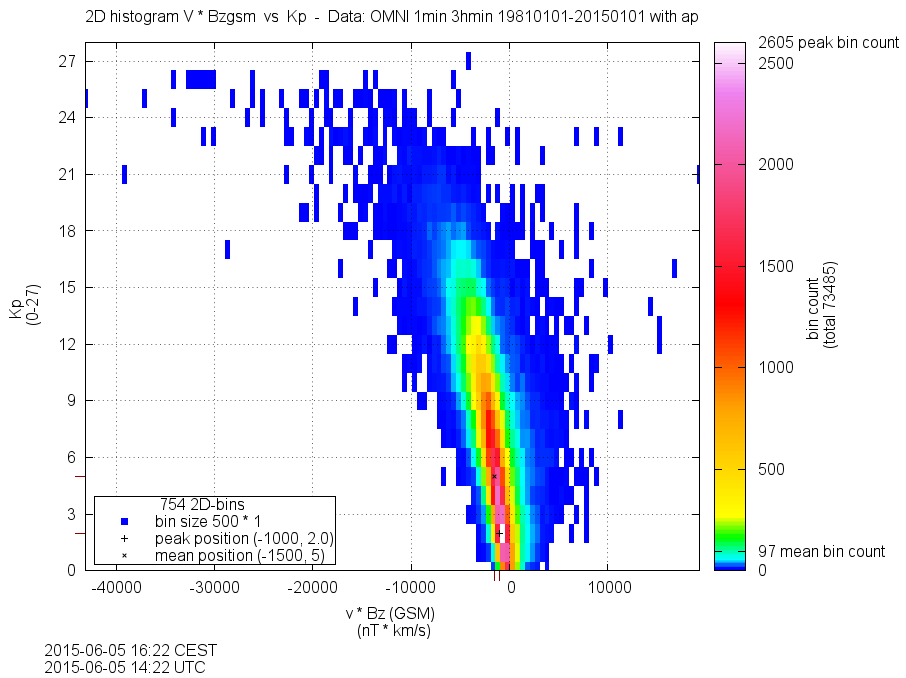
\includegraphics[width=0.3\textwidth]{images/gnuplots/2Dhistogram_3hmin_VBzgsmvsKp_new_plot.png}
	\caption{Plot fo Kp frequency by V*Bzgsm. make plot flatter...}
	\label{fig:2Dhistogram_3hmin_VBzgsmvsKp_new_plot}
\end{figure}

correlation coefficient...\\

VBzgsmvsKp dependence plot; V shape\\
see \autoref{fig:2Dhistogram_3hmin_VBzgsmvsKp_new_dependence_plot}
\begin{figure}[htb]
	\centering
	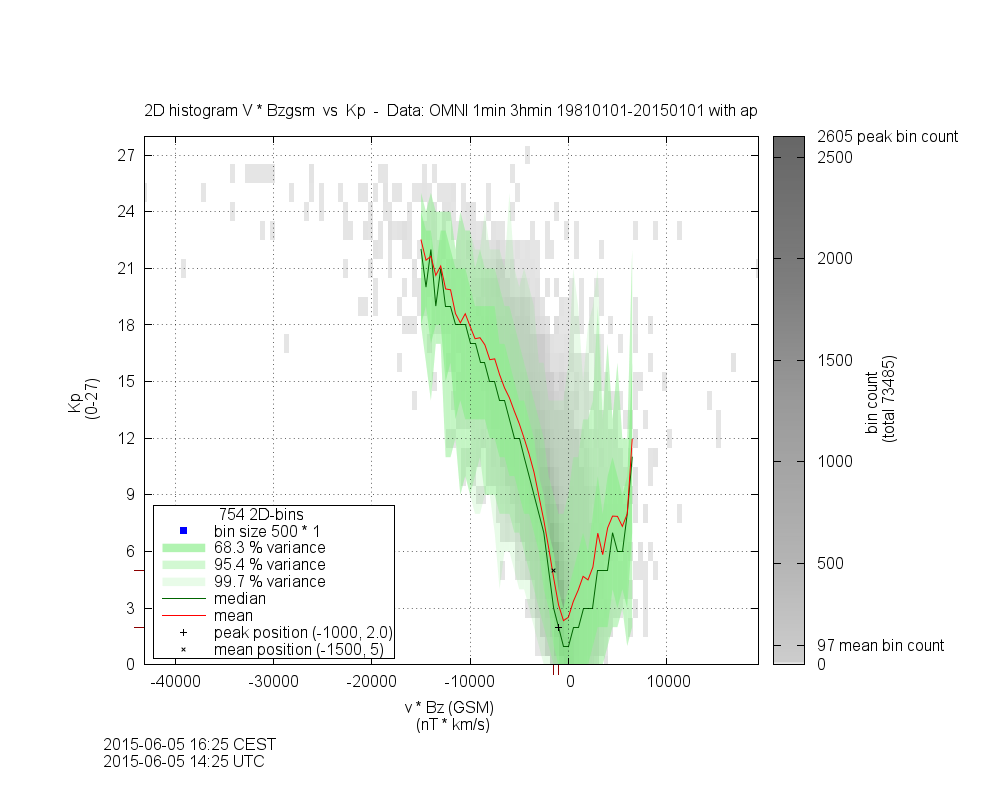
\includegraphics[width=0.3\textwidth]{images/gnuplots/2Dhistogram_3hmin_VBzgsmvsKp_new_dependence_plot.png}
	\caption{Plot like Figure~XX but with the Kp dependency.}
	\label{fig:2Dhistogram_3hmin_VBzgsmvsKp_new_dependence_plot}
\end{figure}

Results of this section.\\
What kind of solar wind structures create the individual regions in this distribution? -> next section\\
What is their individual contribution to the Kp ranges (e.g. high Kp: CMEs 70\% and CIRs 30\%)? -> next section\\

maybe correlation coefficient frequency spectra over time...?\\


\section{Solar wind structure type influence on the terrestrial magnetosphere}

How strong do different structure types influence the terrestrial magnetosphere?\\

present single events, avg solar wind and CME\\
show for both VBzgsmvsKp plot

sws23 VBzgsmvsKp see \autoref{fig:OMNI_HRO_1MIN_19810101-20130731_with_ap_vBzgsm_3hmin_sws23_VBzgsmvsKp_2Dhistogram_plot}
\begin{figure}[htb]
	\centering
	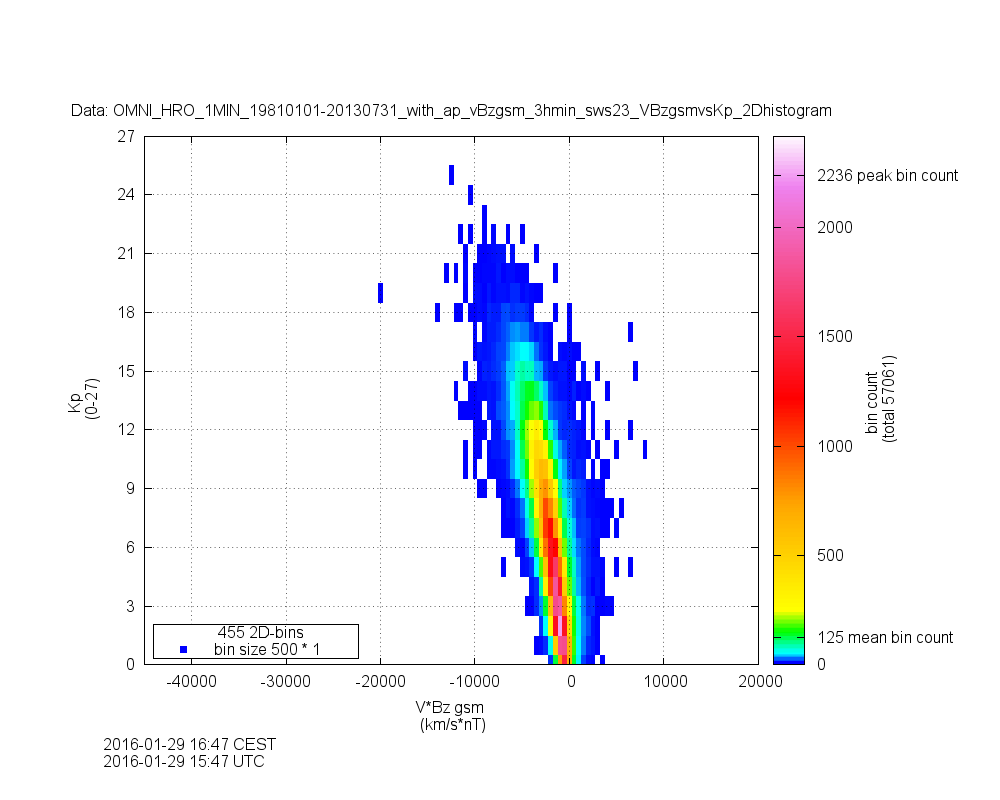
\includegraphics[width=0.3\textwidth]{images/gnuplots/OMNI_HRO_1MIN_19810101-20130731_with_ap_vBzgsm_3hmin_sws23_VBzgsmvsKp_2Dhistogram_plot.png}
	\caption{same as Figure~XX... with the non-CME data flagged by the solar wind structure list. sws23 VBzgsmvsKp}
	\label{fig:OMNI_HRO_1MIN_19810101-20130731_with_ap_vBzgsm_3hmin_sws23_VBzgsmvsKp_2Dhistogram_plot}
\end{figure}

sws1 VBzgsmvsKp see \autoref{fig:OMNI_HRO_1MIN_19810101-20130731_with_ap_vBzgsm_3hmin_sws1_VBzgsmvsKp_2Dhistogram_plot}
\begin{figure}[htb]
	\centering
	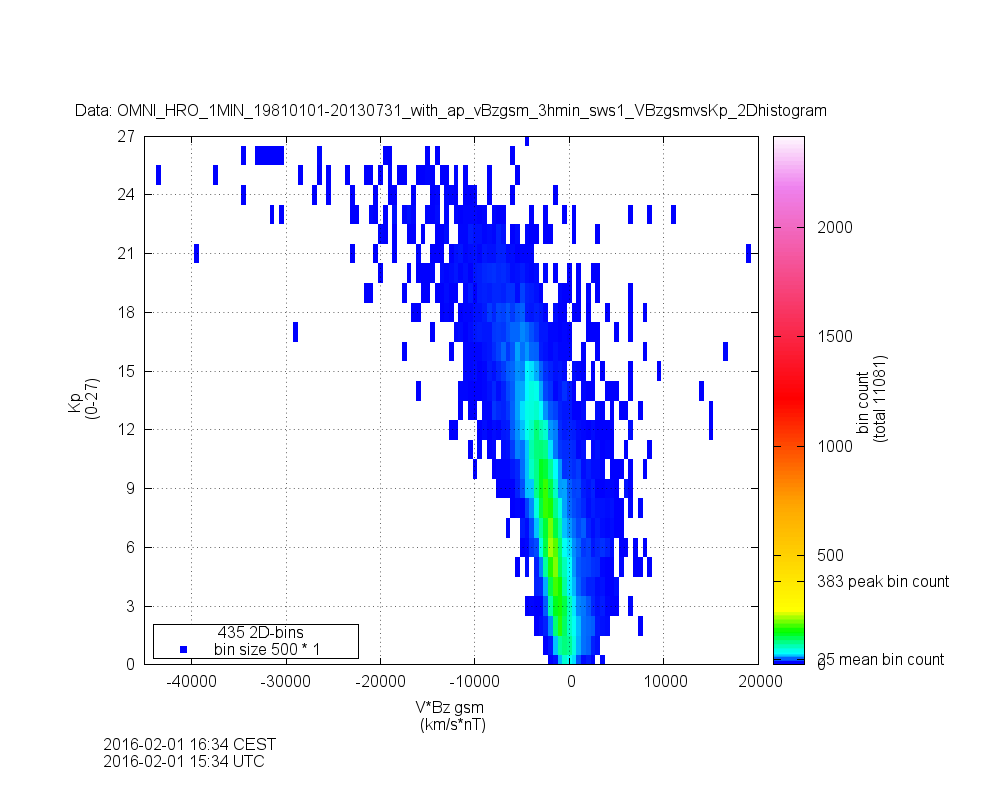
\includegraphics[width=0.3\textwidth]{images/gnuplots/OMNI_HRO_1MIN_19810101-20130731_with_ap_vBzgsm_3hmin_sws1_VBzgsmvsKp_2Dhistogram_plot.png}
	\caption{same as Figure~XX... with the CME data flagged by the solar wind structure list. sws1 VBzgsmvsKp}
	\label{fig:OMNI_HRO_1MIN_19810101-20130731_with_ap_vBzgsm_3hmin_sws1_VBzgsmvsKp_2Dhistogram_plot}
\end{figure}

CME- and non-CME 'comparison' see \autoref{fig:OMNI_HRO_1MIN_19810101-20130731_with_ap_vBzgsm_3hmin_sws_VBzgsmvsKp_comparison_plot}
\begin{figure}[htb]
	\centering
	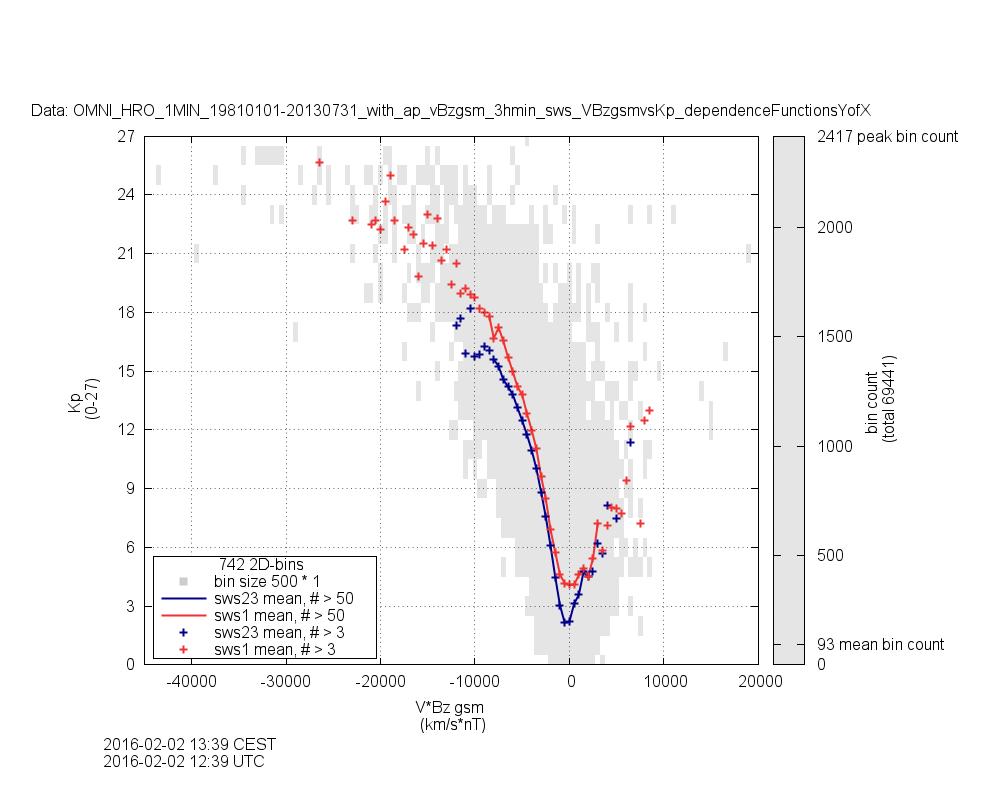
\includegraphics[width=0.3\textwidth]{images/gnuplots/OMNI_HRO_1MIN_19810101-20130731_with_ap_vBzgsm_3hmin_sws_VBzgsmvsKp_comparison_plot.png}
	\caption{Kp dependence on CME- and non-CME structures.}
	\label{fig:OMNI_HRO_1MIN_19810101-20130731_with_ap_vBzgsm_3hmin_sws_VBzgsmvsKp_comparison_plot}
\end{figure}



Kp vs VBzgsm - CMEs as fraction of overall solar wind; see \autoref{fig:OMNI_HRO_1MIN_19810101-20130731_with_ap_vBzgsm_3hmin_CMEpart_VBzgsmvsKp_2Dhistogram_plot}
\begin{figure}[htb]
	\centering
	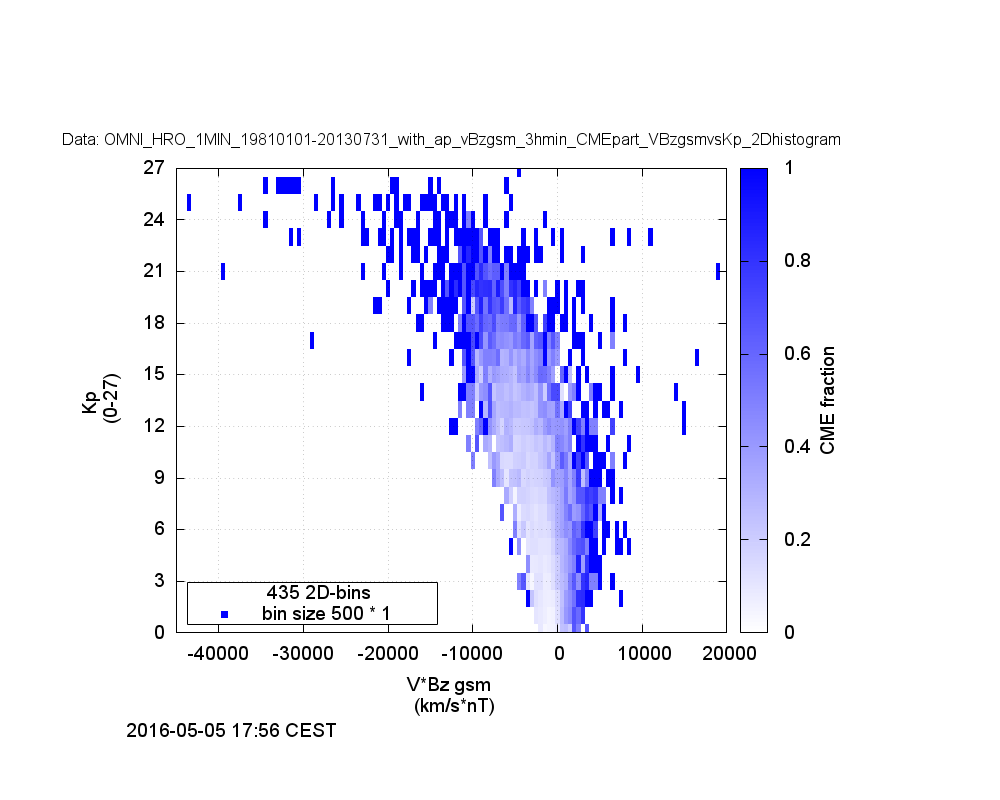
\includegraphics[width=0.3\textwidth]{images/gnuplots/OMNI_HRO_1MIN_19810101-20130731_with_ap_vBzgsm_3hmin_CMEpart_VBzgsmvsKp_2Dhistogram_plot.png}
	\caption{CMEs as fraction of overall solar wind. sws1/sws}
	\label{fig:OMNI_HRO_1MIN_19810101-20130731_with_ap_vBzgsm_3hmin_CMEpart_VBzgsmvsKp_2Dhistogram_plot}
\end{figure}


\section{Solar wind structure analyses}
%\label{sec:}

ACE solar wind time series (at 1\,au) and event list\\

see OPTIMAP events\\
?to analyse: ACE event lists\\
%method: automatic list creation by event detection via parameter thresholds

sample CME analyses (MVA, -> Kp)\\


\section{CME impact on the magnetosphere}

analyze sw coupling to the magnetosphere for being able to estimate CME impact from white light images (see paper draft...)\\

events from ACE CME list...\\

add OMNI ap->Kp values and sws flags\\
filter to sws1 and sws23 data\\
compare CME vs non-CME distributions (VBzgsmvsKp, VvsKp, BvsKp, BzgsmvsKp..)\\
get dependence functions\\


\section{Solar wind frequency distributions}

How often occur certain conditions?\\

OMNI hourly data\\
$v, B, T, n$\\
see \autoref{fig:histogram_V_plot}
%do all four figures...
\begin{figure}[htb]
	\centering
	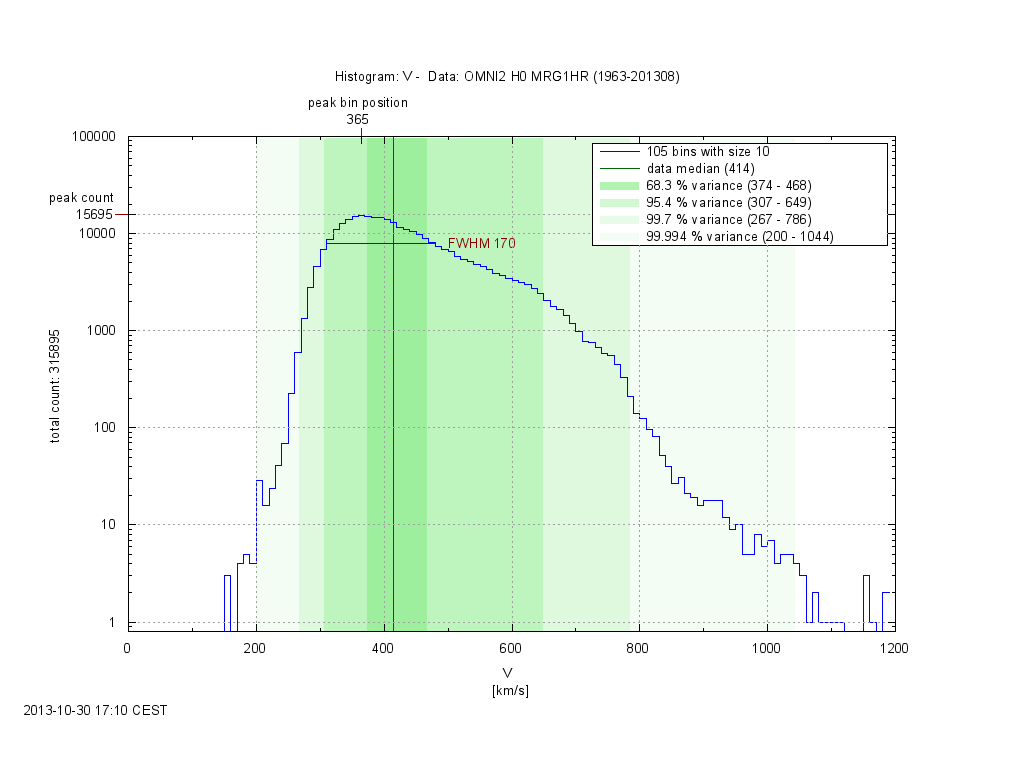
\includegraphics[width=0.3\textwidth]{images/gnuplots/histogram_V_plot.png}
	\caption{Histogram of solar wind velocity.}
	\label{fig:histogram_V_plot}
\end{figure}

%maybe couple with solar wind model...?\\

- overall frequency\\
- variation over the years (solar cycle)\\
- seasonal variation\\
- internal variation (HSS, LSS, CMEs)\\


\subsection{Solar wind solar cycle dependence}

%definition of 4 solar cycle phases?\\
%cycle dates: min, rise, max, set (maybe omit this?)\\

the density shows no obvious solar cycle dependence (look into it...)\\
the parameters V, T and B show a clear solar cycle dependence\\
see \autoref{fig:OMNI_yearly_freq_NVTBSSN_gps}
\begin{figure}[htb]
	\centering
	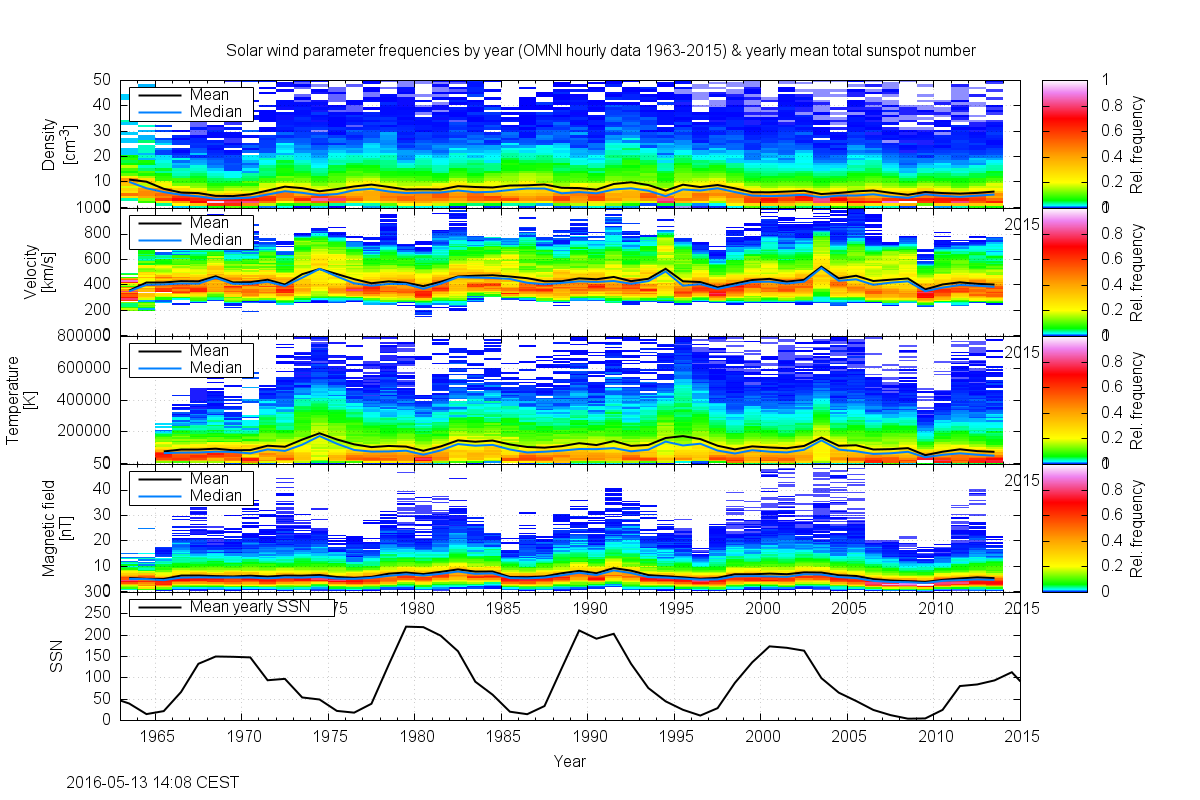
\includegraphics[width=0.3\textwidth]{images/gnuplots/OMNI_yearly_freq_NVTBSSN_gps.png}
	\caption{Plot of solar wind parameter frequencies and mean total sunspot number by year for the period 1963--2013. Density, velocity, temperature and magnetic field frequencies show more or less a solar cycle dependence, illustrated by the mean total sunspot number. SSN data from WDC-SILSO, Royal Observatory of Belgium, Brussels.}
	\label{fig:OMNI_yearly_freq_NVTBSSN_gps}
\end{figure}
add SSN matrix plot...\\


\subsection{Solar wind seasonal dependence}

seasonal variation\\
sw by month\\
quantify variation amplitudes\\

see \autoref{fig:OMNI_monthly_freq_V_gps}
%do all four figures...
\begin{figure}[htb]
	\centering
	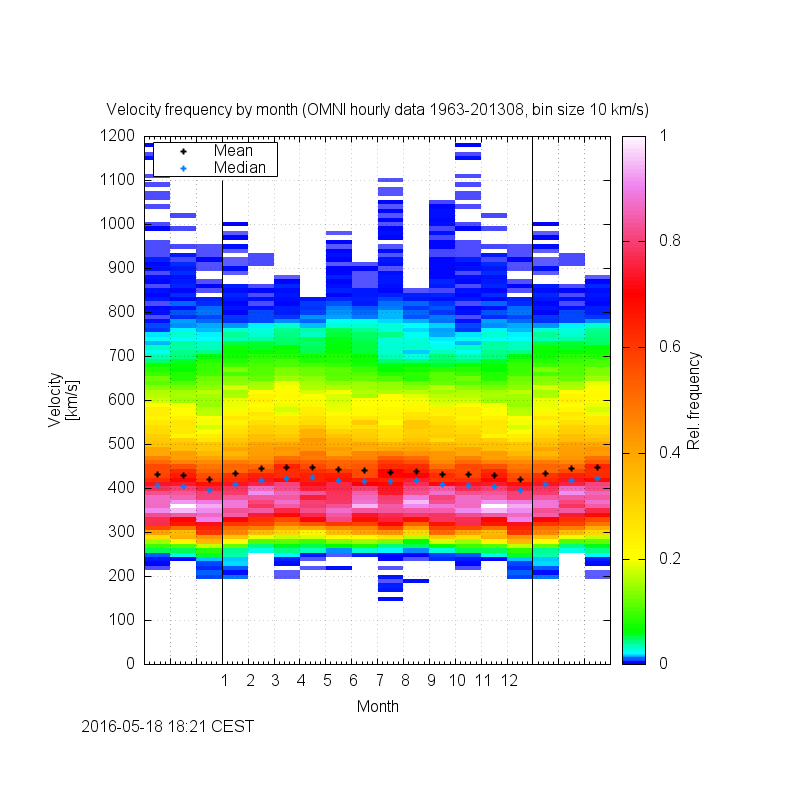
\includegraphics[width=0.3\textwidth]{images/gnuplots/OMNI_monthly_freq_V_gps.png}
	\caption{Diagram of the velocity frequency by month for the period 1963/01--2013/08. Mean and median values are shown as well.}
	\label{fig:OMNI_monthly_freq_V_gps}
\end{figure}


derived exponent values from simple trigonometric fit on monthly values:\\
$c_N = -2.234$\\
maybe figure?\\

...following maybe into section 'radial dependence of median value?\\
expected influence from perihelion/aphelion (see Appendix...) distance vs observations\\
we expect for the proton density (scaling law $N(r) = 7.6~\text{cm}^{-3} \cdot r^{-2}$):\\
N(0.983~au) = 7.9~cm$^{-3}$\\
N(1~au) = 7.6~cm$^{-3}$\\
N(1.017~au) = 7.3~cm$^{-3}$\\
we expect for the magnetic field strength (scaling law $\propto r^{-1.6}$):\\
B(0.983~au) = 6.3~nT\\
B(1~au) = 6.1~nT\\
B(1.017~au) = 5.9~nT\\


see \autoref{fig:OMNI_monthly_freq_B_a_gps}
%do all four figures...
\begin{figure}[htb]
	\centering
	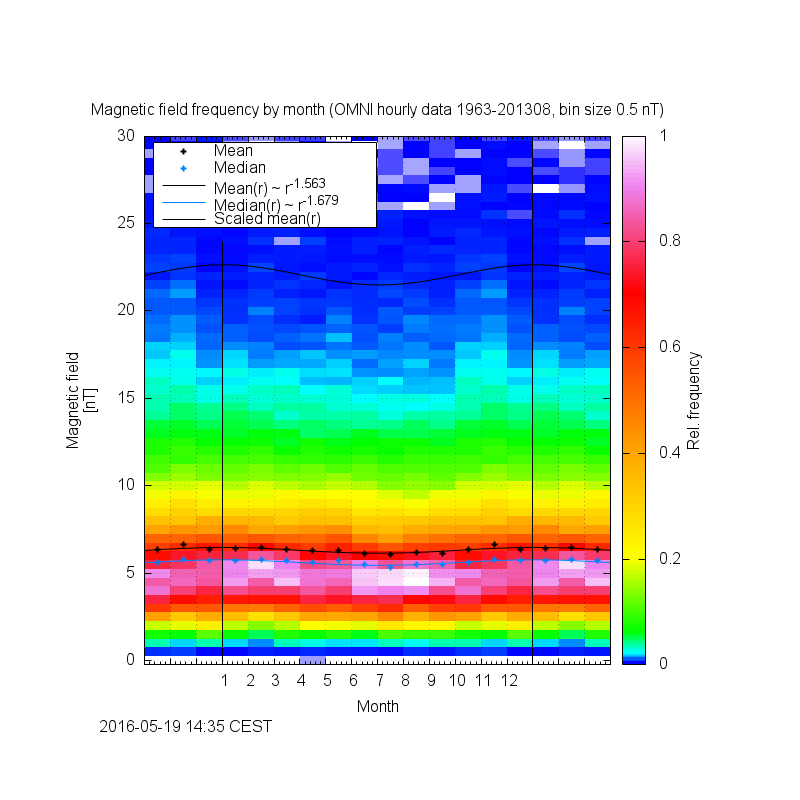
\includegraphics[width=0.3\textwidth]{images/gnuplots/OMNI_monthly_freq_B_a_gps.png}
	\caption{Diagram of magnetic field frequency by month for the period 1963/01--2013/08. Mean and median values are shown as well as the expected course from the solar distance variation (obtained from Helios data).}
	\label{fig:OMNI_monthly_freq_B_a_gps}
\end{figure}


\section{Kp frequency distribution}

Plot of the Kp frequency distribution (see \autoref{fig:histogram_Kp_plot})	%make better than VBTp129!
\begin{figure}[htb]
	\centering
	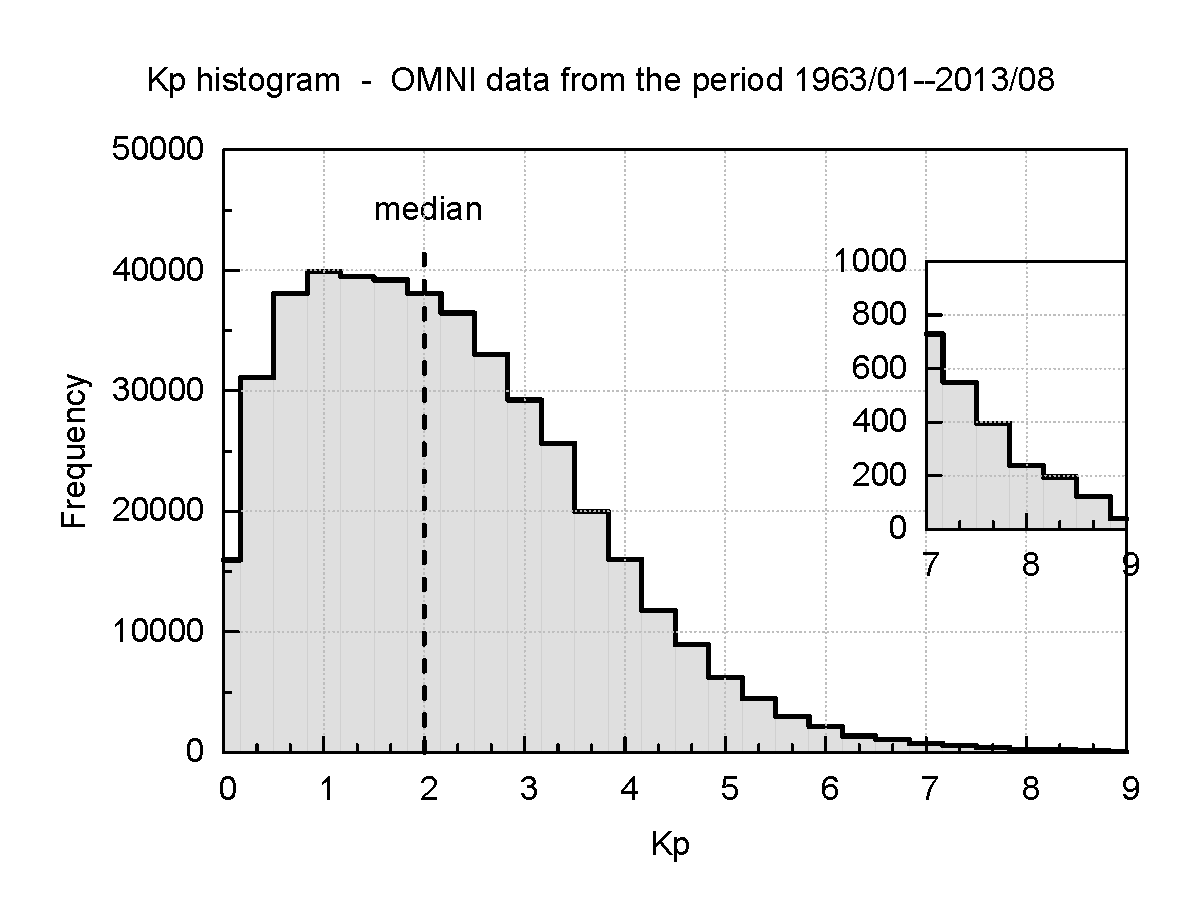
\includegraphics[width=0.3\textwidth]{images/gnuplots/histogram_Kp_plot.pdf}
	\caption{Kp frequency distribution for the period 1963/01--2013/08. The median Kp value is 2 and a Kp of 9o occurred only 39 times. OMNI data.}
	\label{fig:histogram_Kp_plot}
\end{figure}


\subsection{Kp solar cycle dependence}
%\label{sec:}

%cycle dates: min, rise, max, set (maybe omit this?)\\

- solar cycle variations\\
- variations between solar cycles\\

the yearly Kp frequency shows variations; the yearly mean Kp shifts about 2~units.\\
plot of the yearly Kp frequency (see \autoref{fig:Kp_freq_yearly_ssn_plot})
\begin{figure}[htb]
	\centering
	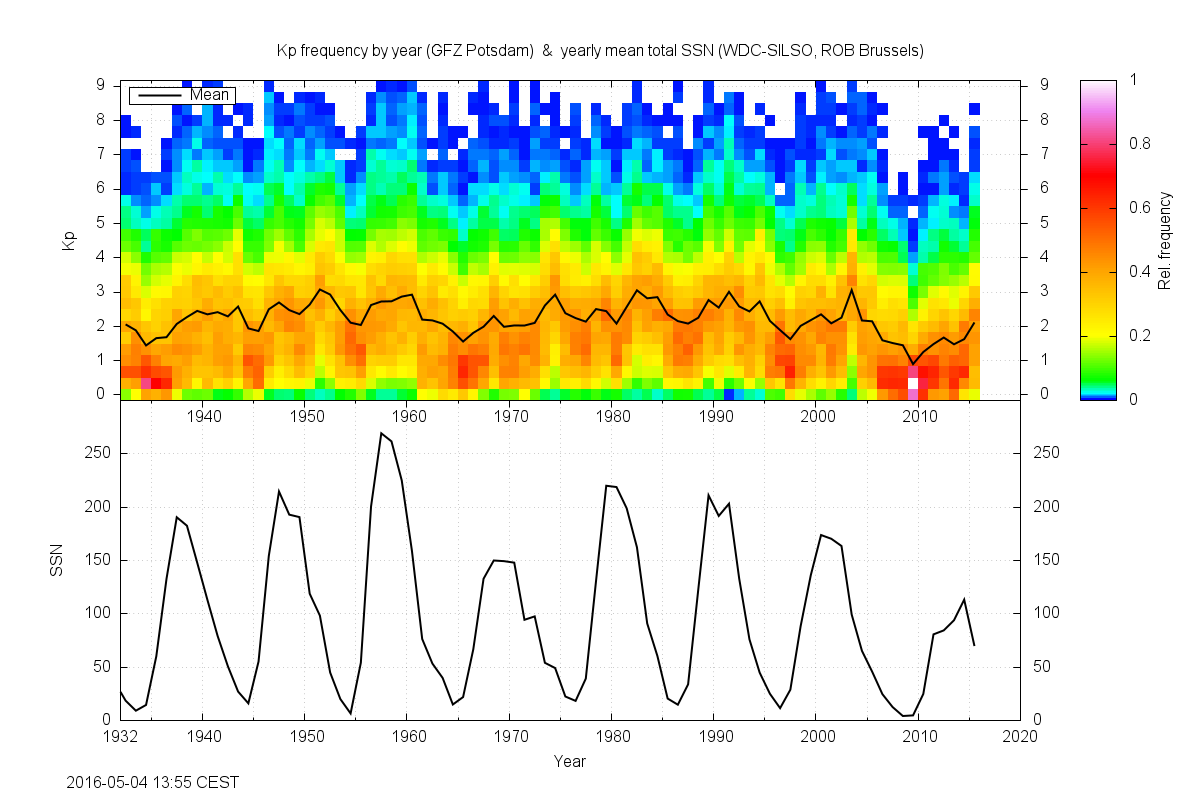
\includegraphics[width=0.3\textwidth]{images/gnuplots/Kp_freq_yearly_ssn_plot.png}
	\caption{Kp frequency by year, yearly mean Kp and yearly mean total SSN for the years 1932--2015. The pattern of Kp shows an imprint of the solar cycle. Kp data from GFZ German Research Centre for Geosciences, Potsdam, Germany and SSN data from WDC-SILSO, Royal Observatory of Belgium, Brussels.}
	\label{fig:Kp_freq_yearly_ssn_plot}
\end{figure}
add Kp--SSN matrix plot...\\

analyze Kp frequency by month for different SWSs\\
analyze Kp frequency by year for different SWSs\\
put into later part of analysis...


\subsection{Kp seasonal dependence}
%\label{sec:}

for high Kp values (>~4?) there are yearly frequency maxima at the equinoxes and minima at the solstices. this variation amounts to more than 1~Kp (see \autoref{fig:Kp_freq_monthly_plot})
\begin{figure}[htb]
	\centering
	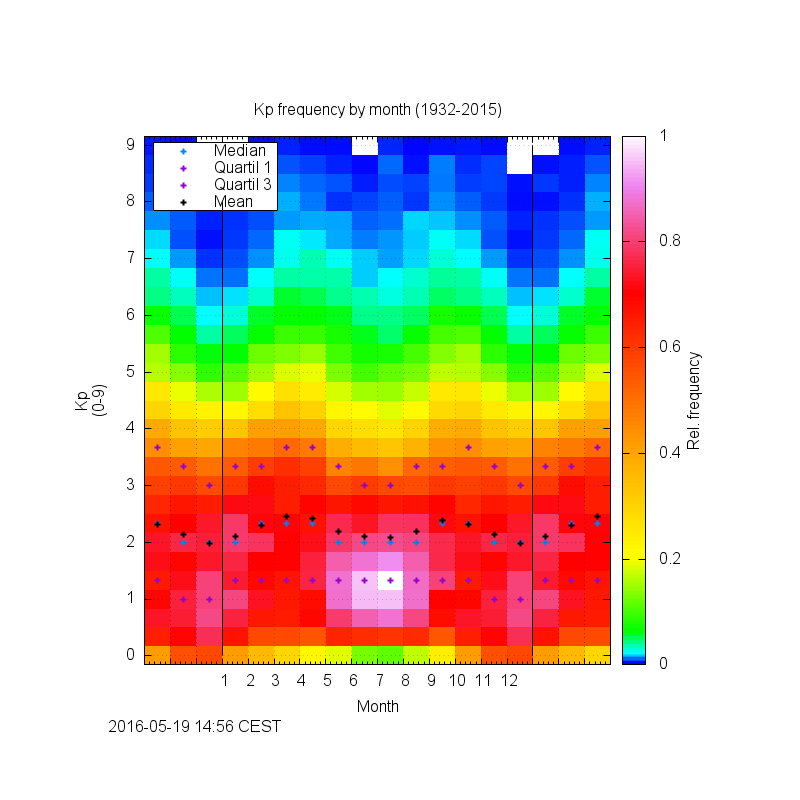
\includegraphics[width=0.3\textwidth]{images/gnuplots/Kp_freq_monthly_plot.png}
	\caption{Diagram of Kp frequency by month for the period 1932--2015. Median and quartil values are shown as well. remove mean...}
	\label{fig:Kp_freq_monthly_plot}
\end{figure}

possible causes (see \citet{Rangarajan1997} p. 1282 and mention Bartels1963 too
):\\
- Earth's rotation axis tilt ($\pm23.44$\textdegree) (obliquity to orbit/inclination of equator)\\
- solar rotation axis tilt ($\pm7.25$\textdegree) (cite 'NASA Earth fact sheet')\\
- varying distance from Sun 0.983--1.0167~au ($\pm3.3~\%$)\\
- changing solar cycle polarity gives two superimposed maxima... -> No. see even/odd plots\\

read Bothmer1998 Ch 3...\\


\section{Summary/Results}

sw-nowcast: vBzgsm-Kp relation (average and worst case)\\
CME-forecast: v-Kp relation (average and worst case)\\

seasonal correction: $\Delta$Kp(month)\\
$Kp_\text{impact} = Kp_\text{CME} \pm \Delta Kp(month)$\\

sw-timeseries ACE OPTIMAP ``Zeitreihe''-events

\section{Forecast}
%\label{sec:}

\subsection{Internal solar wind correlations}

B-V correlation\\
ACE MAGSWE 64~s data -> yearly overlay plot\\


\subsection{Kp forecast from CME velocity}

V-Kp correlation\\
similar to \citet{Elliott2013}; different data resolution and averaging method (3-hour maximum of 1~min data)

\section{Applications}

rssfeeds, rtsw plots\\
CME Kp impact\\
part of DDC\\


%%%%%%%%%%%%%%%%%%%- Solar wind evolution -%%%%%%%%%%%%%%%%%%%%%%%%

\chapter{Solar wind origin and evolution}
%\chapter{}

%COFI -- chapter outline and flow integration\\

talk about origin and evolution...\\

what is the aim?\\
- empirical analytical sw distribution model with radial dependence\\
- sw extrapolation to near-Sun region with an empirical sw model\\

Motivation?\\
- solar wind acceleration\\
- coronal heating problem\\
- SPP mission\\

new analyses of the Helios solar wind data\\

input (Helios data):\\
	magnetic field strength; proton velocity, number density and temperature\\

output (results):\\
	empirical distribution model for 0.29--0.98~au\\
	empirical distribution extrapolation model to near-Sun region\\
	L-> refined models with the combination of OMNI data\\
	
theory/literature:\\
existing model: \citep{Sittler1999}\\
L-> compare with their radial density function eq. (18a)\\
existing solar wind and CME measurements, steady state mass flow (eq.~(5)), velocity model v(r) \citep{Sheeley1997}\\
Helios results, radial gradients see Schwenn1990 p.~155\\
Schwenn1983 intro -> sw-averaging comment (beer and wine)\\)

\citet{Balogh1999} (origin and formation of CIRs in inner heliosphere with Helios data)\\

%see astro70/CGAUSS/dropbox_presis/...\\

see Hellinger2013 p.1353\\
see Balogh1999 from p. 162\\
and what differentiates our model from the others...\\\

model constraints:\\
see Marsch1999...\\

%see presi 1.07 Inside Helios-Origins and Evolution-Salem.ppt


\section{Solar wind parameters}	%for the region below 1~au

%Methods:
% 2016-08-28
% 	determine fit function type for radial dependency of Helios data
%		-> exponential regression fit
%		=> data mean(r) and median(r)
%	determine fit function type for frequency distribution of 1~au OMNI data
%		-> lognormal fit
%		-> double lognormal fit
%		=> weight parameter c
%	build exponential radial double lognormal function
%		-> fit that function to the radial frequency binned data
%		=> fit parameters define Helios sw model for [0.3--1~au]
%	evaluation of function behavior in direction of Sun up to 0.04~au
%		-> extrapolation not feasible with variable width -> constant width (constant sigma/shape)
%		-> single lognormal function sufficient; see WSSR
%	single lognormal fit with constant width
%		-> extrapolation model
%
%	Model variants:
%	- Helios replication model [0.3--1~au]
%	- Helios extrapolation model [0.04--1~au]
%	OMNI 1~au median (mean?) value of specified period:
%	- all-time extrapolation model (mean model with whole OMNI period)
%	- current extrapolation model (current year median or so)
%	- forecast extrapolation model (that years solar cycle historic median)
%
%	boundary conditions:
%	- 1~au OMNI data
%	- continuity of mass flux


motivation/reason for necessity?/why?\\

which parameters? (major solar wind parameters)\\
- The characteristic behavior of a plasma is determined by its density, temperature and magnetic field strength. cite?\\
- the velocity is the defining parameter of the solar wind\\

definition of 'the four solar wind parameters':\\	%by OMNI histograms
	magnetic field strength, aka magnetic field, $B$, usually measured in nT, in the order of 0--35~nT at 1~au\\
	proton bulk velocity, aka velocity, $v$, usually measured in km/s, in the order of 200--900~km/s at 1~au\\
	proton number density, aka density, $n$, usually measured in cm$^{-3}$, in the order of 1--60 at 1~au\\
	proton temperature, aka temperature, $T$, usually measured in K, in the order of 10\,000--1\,000\,000~K at 1~au\\
sentence about ordering of the parameters...\\


%data binning
hourly OMNI data\\
measurement precision:\\
$B$: 0.01~nT\\
$v$: 1~km/s\\
$n$: 0.1~cm$^{-3}$\\
$T$: 1~K ? (smallest found: 7~K)\\

error discussion:\\
OMNI hourly data mean:\\
$B$: bin size 0.5~nT, median 5.6, mean 6.30056(18)\\
$v$: bin size 10~km/s, median 414, mean 437.6700(18)\\
$n$: bin size 1~cm$^{-3}$, median 5.3, mean 6.831410(18)\\
$T$: bin size 10\,000~K, median 80\,751, mean 112\,219.0(19) (with 1000~K as precision)\\

empirical data; Helios; hourly\\
why hourly and not higher resolution data?\\
measurement precision:\\
$B$: 0.01~nT\\
$v$: 0.1~km/s\\
$n$: 0.1~cm$^{-3}$\\
$T$: 100--1000~K (3 digits)\\
$r$: 0.01~au\\

error discussion:\\
Helios hourly data mean:\\
$B$: min 337, precision: 0.000545; 18.3x better\\
$v$: min 497, precision: 0.00449; 22.2x\\
$n$: min 497, precision:  0.00449; 22.2x\\
$T$: min 497, precision: 4.49--44.49 22.2x\\
=> so we use 1/10 the measurement precicion for the mean.\\

median precision same as data precision\\


\section{Empirical solar wind model}

Helios data ranges:\\
- time range [1974-12-10--1980-03-04]\\
- solar distance range 0.29--0.98~au\\
- 0°--360° longitude\\
- latitude range -7.25°--7.25°\\
data constrictions:\\
- hourly data\\
- data gaps -> uneven coverage -> solar cycle minimum dominates\\
- limited parameter ranges\\

model boundaries (spherical coordinates):\\
- mean solar wind of the Helios time range\\
- solar distance range 0.29--0.98~au\\
- rotational symmetry\\
- confined to ecliptic\\
model constrictions:\\
- radial dependency function\\
- frequency distribution function\\

all assumptions outside these boundaries are extrapolations with large uncertainties...\\

%latitude variation negligible?
influence from latitude variation in data negligible? (see Ulysses figure in introduction). Helios probes within ecliptic => variation span equal to solar tilt: -7.25° to 7.25°; solar tilt/obliquity to ecliptic: $i_\odot = 7.25\degree$ (Sun fact sheet: \url{http://nssdc.gsfc.nasa.gov/planetary/factsheet/sunfact.html)}\\
big part of Helios data is from latitudes $>\pm5$°, see Figure~XX (data count over latitude) and see Figure~XX (Helios orbit polar plane in data section...)\\
As we see at the end of this chapter in Section~XX, the latitude influence is negligible and so we assume it to be constant for our models.\\
see also \citet{Richardson1995}\\
see also \citet{Schwenn1990} p.~127\\

%%%%%%%%%%%%%%%%%%%%%%%%%%
approach:
\begin{itemize*}
	\item determine fit function type for radial dependency of Helios data
	\item determine fit function type for frequency distribution of OMNI data
	\item fit exponential radial double lognormal function to binned Helios data
	\item evaluation of function behavior in direction of Sun up to 0.04~au
	\item single lognormal fit with constant width is extrapolation model
	\item model evaluation
	\item some model variants with OMNI median values
\end{itemize*}


\subsection{Solar distance dependency---theory}
%\label{sec:}

%why both median and mean?\\

heliospheric distance $r$\\
averages: median(r), mean(r)\\

solar wind parameter distributions and their radial dependence from theory/literature:\\
B-field radial profile: $B \propto r^{-.5?}$\\
	Kivelson/Parker references\\
	shear effect from solar rotation; talk 2014-07-21\\
velocity radial profile: $V \propto r^{0?}$\\
	model based on LeBlanc1998 electron density with flux conservation: Zic2015(Temmer)\\
	Parker...\\
density radial profile: $N \propto r^{-2}$\\
	simple view: for a spherical constant velocity mass outflow a one over distance squared law is expected because of the mass flux conservation per solid angle for different distances. measurements up to the outer heliosphere confirm the $1/r^2$ dependency (1--38~au by Voyager~2, \citep{Belcher1993} newer paper?)\\
	electron density model corona--1~au LeBlanc1998\\
	radial electron density from Helios $6.14r^-2.10$ compared to radio bursts see Bougeret1983\\% (not Bothmer1998 and not Schwenn1990 book)\\
	existing electron density model see Leblanc1998\\

	in an ideal neutral plasma the electron and proton number density have the same values (neutral plasma) (reference?)\\
	ca. 10~\% more electrons than protons (due to alphas) cite?\\	%http://omniweb.gsfc.nasa.gov/ftpbrowser/bow_derivation.html\\
	radial electron density models suggest a proportionality to $r^{-2}$ for $r > 10~R_\odot$ (leblanc1998 with its Figure~6)\\
temperature radial profile: $T \propto r^{-1?}$\\
	at larger distances heating outbalances the adiabatic temperature part (adiabatic cooling vs. pickup proton and stream--interaction heating; 1--68~au by Voyager~2; \citet{Richardson2003}\\


solar wind ram pressure $p_\text{ram} = \rho V^2$\\

conserved quantities:\\
- momentum conservation... VBbookp112\\
- flux conservation...\\

%%%%%%%%%%%--  flux  --%%%%%%%%%%%%%%%
%As Schwenn1983 stated ``From Helios in situ measurements we know that at least beyond 0.29~au there is almost no nonradial flow, on the average. In fact, the particle flux was found to be that quantity which varies the least with increasing R.''\\

%Schwenn1990:
%increase in sw velocity with distance; speed increase mainly in slow solar wind
%density deviates from a purely r^-2 fall-off (10% faster); n(r)=6.1*r^-2.1 cm^-3; different behavior in slow and fast wind
%proton flux density constant between 0.3-1.0~au -> no meridional flow into/out of the ecliptic; different for slow and fast sw

With consideration of continuity the mass flux per solid angle has to be constant: $\dot{m} = \text{const}$\\
conserved quantities:\\
- mass flux: $\dot{m} = \rho v A$ (with mass density $\rho$, velocity $v$ and [cross-sectional area $A$] or solid angle?...)\\
- particle fluxes (proton flux, electron flux, etc.)\\
	- proton flux: $j_\text{p} = n_\text{p} v_\text{p} A$ (with proton density $n_\text{p}$ and proton velocity $v_\text{p}$)\\

(with proton mass density $\rho = n_\text{p} m_\text{p}$ (with proton number density $n_\text{p}$ and proton mass $m_\text{p}$).)\\

the individual radial dependencies for a spherical radial outflow are:\\
$A(r) \propto r^2$ --> $A/r^2 = \text{const}$\\
and assuming an exponential dependency,\\
$n_{\text{p}}(r) = n_0 r^{c_n}$,\\
$v(r) = v_0 r^{c_v}$\\
\begin{align}
	j_\text{p} &= \text{const}\\
	n_\text{p} v_\text{p} A &= \text{const}\\
	n_0 r^{c_n} v_0 r^{c_v} r^2 &= \text{const}\\
	r^{c_n} r^{c_v} r^2 &= \text{const}\\
	\Rightarrow c_n + c_v + 2 &= 0\\
	c_n + c_v &= -2
\end{align}
an increasing velocity should result in a steeper density...\\

validity of mass flux continuity: within the heliosphere mass to energy conversion and vice versa is negligible, but there can be flux from and to higher latitudes as the Helios data is localized to a small latitude range in the ecliptic plane.\\
estimate the error from that... (if error is too big => drop continuity condition)\\
larger errors should be located near CMEs and CIRs (nonradial flows from interactions)\\
there is a proton flux difference between slow and fast solar wind streams (see book Schwenn1990 p.~146)

estimate the possible size of error:\\
mean:\\
$c_n = -2.010$\\
$c_v = 0.049$\\
$c_n + c_v = -1.961$\\
difference to -2 is 0.039\\
% [median:\\
% $c_n = -2.093$\\
% $c_v = 0.058$\\
% $c_n + c_v = -2.035$\\
% difference to -2 is -0.035\\
% ]constant mass flux only for mean...\\


\subsection{Solar distance dependency---Helios data}

we want to obtain the solar distance dependence of the mean and the median of the Helios data\\

%data
we use hourly Helios data...\\
the hourly Helios data has a native radial resolution of 0.01~au, so for calculating the median the data is binned into 0.01~au bins\\

%why exponential function?
we expect an exponential behavior from all four parameters (see radial dependence theory section with literature references)\\
=> therefore we use an exponential regression fit function $f(r) = a\,r^b$.\\
fit weighting by counts per bin\\

%fit result figures
the resulting fit curves are displayed in \autoref{fig:radial_fit_4_thesis_pdfcairo_plot}. Larger individual Graphs can be found in the appandix (Figures~XX).%\ref{fig:radial_fit_Bv_thesis_pdfcairo_plot} and \ref{fig:radial_fit_nT_thesis_pdfcairo_plot}).
\begin{figure}[htb]
	\centering
	\includegraphics[width=1\textwidth]{images/gnuplots/radial_fit_4_thesis_pdfcairo_plot.pdf}
	\caption{Plots of the four solar wind parameters over solar distance. The mean and median per 0.1~au data bin and their fit curves (weighted with data count) are plotted as well.}
	\label{fig:radial_fit_4_thesis_pdfcairo_plot}
\end{figure}

flux figure...\\


%state this at the first occurence... (from GUM guide)
%“mS = 100,021 47(35) g, where the number in parentheses is the numerical value of (the combined standard uncertainty) uc referred to the corresponding last digits of the quoted result.”

%fit result table
With $r$ in astronomical units one gets the fit coefficient values of all four parameters as seen in \autoref{tab:mean_median_fit_parameter}.
\begin{table}[htb]\small
	\centering
	\captionsetup{belowskip=4pt}
	\caption{These are the fit coefficients for the median and mean solar distance dependence functions of the four plasma parameters from the combined Helios data set. The errors in brackets are the estimated standard deviation of each fit parameter. remove units?}
	\begin{tabular}{lrrcrrc}
		\toprule
		\multirow{2}{*}{Parameter}	&\multicolumn{2}{c}{Median}	&	&\multicolumn{2}{c}{Mean}	&mean=median\\
		\cmidrule{2-3}	\cmidrule{5-6}
			&\multicolumn{1}{c}{$a$}	&\multicolumn{1}{c}{$b$}	&	&\multicolumn{1}{c}{$a$}	&\multicolumn{1}{c}{$b$}	&$r_\text{equal}$\\
		\midrule
		Magnetic field	&5.377(92)~nT	&-1.655(17)	&	&6.05(10)~nT		&-1.546(18)	&0.344~au\\
		Velocity	&410.7(28)~km/s	&0.058(13)	&	&435.6(24)~km/s	&0.049(10)	&692~au\\
		Density		&5.61(27)~cm$^{-3}$	&-2.093(46)	&	&7.57(30)~cm$^{-3}$	&-2.010(38)	&0.027~au\\
		Temperature	&7.14(23)$ \times 10^4$~K	&-0.913(39)	&	&9.67(21)$ \times 10^4$~K	&-0.792(28)	&0.081~au\\
		Flux		&fit coeffients...\\
% 		Magnetic field strength	&6.04753	&-1.54631&		&5.37723	&-1.65464	&0.344132483292368\\
% 			&(0.104689)	&(0.0176562)	&	&(0.0919207)	&(0.0171401)\\
% 		Velocity	&435.645	&0.049139	&	&410.72	&0.0580215	&692.392\\
% 			&(2.44896)	&(0.0103927)	&	&(2.81328)	&(0.0127228)\\
% 		Proton density	&7.56767	&-2.00987	&	&5.61317	&-2.09257	&0.027048\\
% 			&(0.300872)	&(0.0384042)	&	&(0.269386)	&(0.0459336)\\
% 		Temperature	&96\,743.2	&-0.792253&		&71\,388.5	&-0.913317	&0.081232928\\
% 			&(2143.64)	&(0.0280191)	&	&(2290.7)	&(0.0389327)\\
		\bottomrule
	\end{tabular}
	\label{tab:mean_median_fit_parameter}
\end{table}
%\captionsetup{width=0.75\textwidth}
%align caption width with table width  OR  widen table to textwidth

skewing of distributions...\\
its change...\\
for the magnetic field strength the mean and median cross each other at 0.344~au.\\


\subsection{Latitude dependency---theory}

refer to Ulysses figure...\\
Ulysses swoops polar plots...\\
see Schwenn1990's~Fig.~3.14\\


\subsection{Latitude dependency---Helios data}

latitude; see \autoref{fig:latitude_frequency_4_thesis_plot}
\begin{figure}[htb]
	\centering
	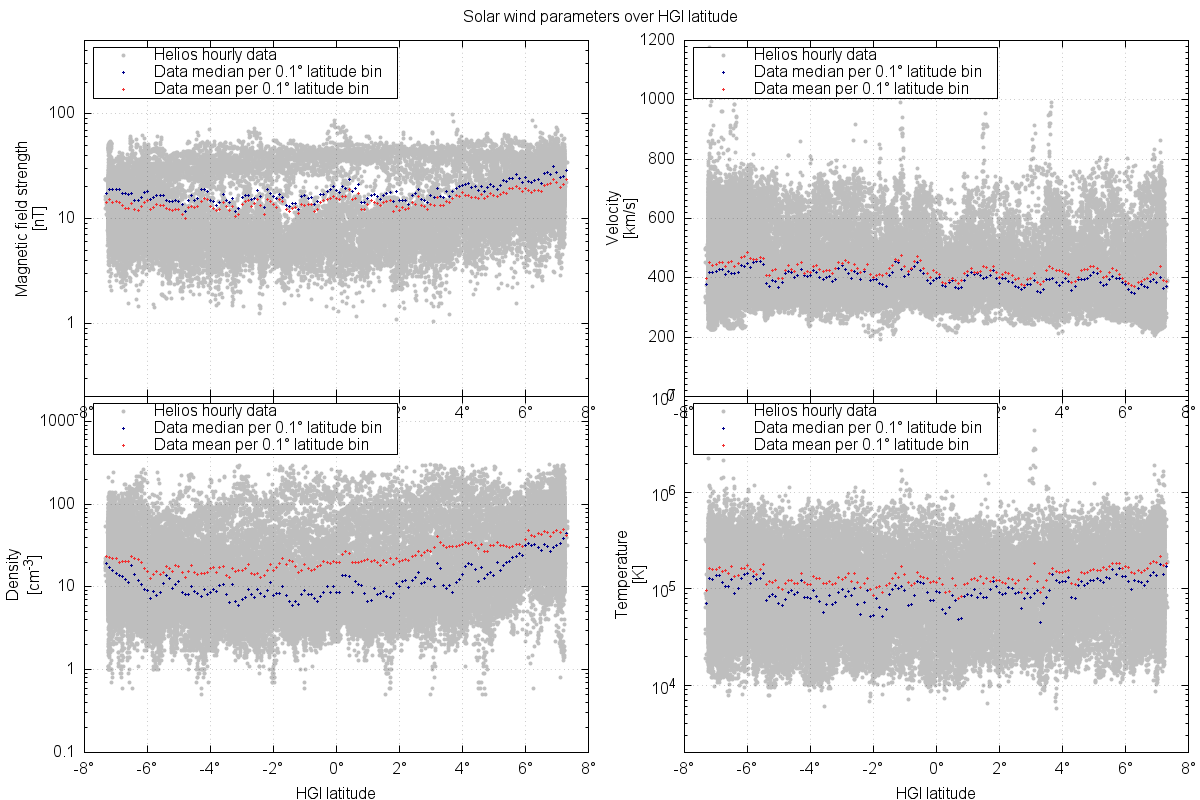
\includegraphics[width=0.5\textwidth]{images/gnuplots/latitude_frequency_4_thesis_plot.png}
	\caption{The four solar wind parameter's HGI latitude dependency. Their mean values per 0.1° bin are plotted as well. make figure same dimensions as projected figure in analysis part...}
	\label{fig:latitude_frequency_4_thesis_plot}
\end{figure}

with the exponential dependencies to 1~au projected solar wind parameters; there are only small changes with latitude in the range -7.25°--7.25°\\
have a look on distribution widths...\\

dependence from latitude in interval -7.25°--7.25° in Helios data negligible?, see \autoref{fig:latitude_frequency_rcorrected_v3_4_thesis_plot}.
\begin{figure}[htb]
	\centering
	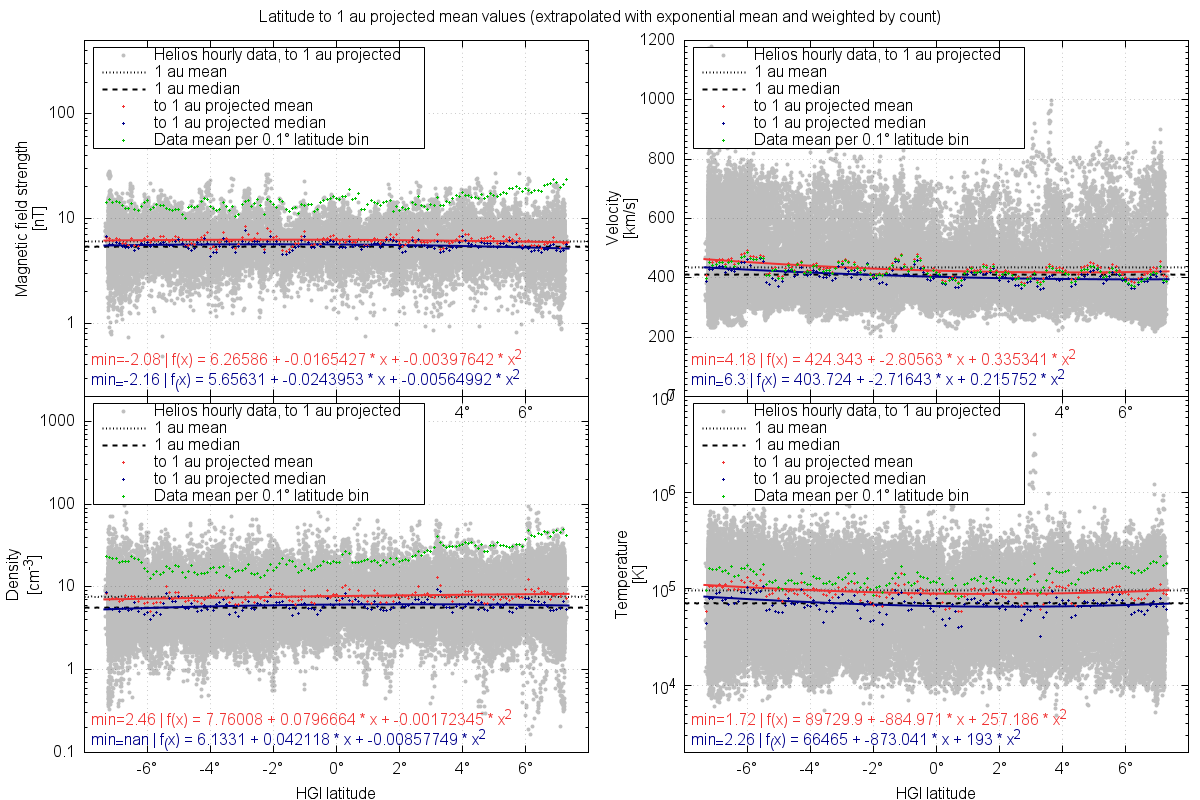
\includegraphics[width=0.5\textwidth]{images/gnuplots/latitude_frequency_rcorrected_v3_4_thesis_plot.png}
	\caption{Plot of the to 1~au projected solar wind parameters over latitude. And their mean values, including weighted fit. add projected median...}
	\label{fig:latitude_frequency_rcorrected_v3_4_thesis_plot}
\end{figure}
estimate error ranges...\\

plot Ulysses data into plot...\\


\subsection{Shape of the frequency distributions}
%\label{sec:}

%aim?
getting shape of the general distributions.\\

%how?
fitting the shape of the parameter's frequency distribution\\

%choice of distribution function?/why lognormal function?\\
Obviously the possible values for all four parameters are positive. This hints to the supposition that they are lognormally distributed, as many positive natural quantities conform to a lognormal distribution. This distribution is described by the lognormal function (For more on lognormal distributions see appendix \autoref{sec:lognormal_distribution}).\\
% * back up with literature references for solar wind parameters AND/OR figure

%fitting method
Therefore we use the lognormal function as a fit function in the process of the least squares regression fitting.\\
%data basis
To evaluate how well the lognormal function represents the solar wind distributions, the abundance of OMNI data (>50~years at 1~au) is more suited than the Helios data (few weeks summed at fixed solar distance), because it enables the averaging over long-time variations like the solar cycle.\\
As basis for the fit in situ solar wind data from the OMNI data set is used (see Section~XX... data section). More precisely, it is hourly data of the whole time range 1963/01--2013/08.\\

%data binning
Helios histogram bin size for mean of frequency distribution (at specific solar distance)\\
$B$: bin size 0.5~nT, min 337, mean precision: 0.000545\\
$v$: bin size 1~cm$^{-3}$, min 497, mean precision: 0.00449\\
$n$: bin size 10~km/s, min 497, mean precision:  0.00449\\
$T$: bin size 10\,000~K, min 497, mean precision: 4.49--44.49\\


\subsubsection{Single lognormal fit}
%single lognormal fit

%fit function
The lognormal fit function
\begin{align}
	W(x) &= \frac{1}{\sigma \sqrt{2 \pi} x} \, \text{e}^{- \frac{(\ln x - \mu)^2}{2 \sigma^2}}	\label{eq:single_lognormal_fit_function}
\end{align}
has two variables, the location ($\mu$) and the shape parameter ($\sigma$) (see also Appendix~XX). The distribution's mean and median postitions are easier to interprete and can directly be calculated from $\mu$ and $\sigma$ (see also Appendix~XX):\\
$median = \text{e}^\mu$\\
$mean = \text{e}^{\left(\mu + \frac{\sigma^2}{2}\right)}$\\
Their values, obtained from the fitting of the four solar wind frequency distributions, are listed in \autoref{tab:single_lognormal_fit_parameters}.
\begin{table}[htb]\small
	\centering
	\captionsetup{belowskip=4pt}
	\caption{These are the resulting fit coefficients $\mu$ and $\sigma$ from the fitting of the lognormal function (\ref{eq:single_lognormal_fit_function}) to the shape of the frequency distributions. The median and mean values and the standard deviation of the fit are shown as well. The values in brackets are the estimated standard deviation of each parameter.}
	\begin{tabular}{lrr.{3.11}.{3.11}.{1.2}}
		\toprule
		Parameter	&\multicolumn{1}{c}{$\mu$}	&\multicolumn{1}{c}{$\sigma$}	&\multicolumn{1}{c}{Median\up{a}}	&\multicolumn{1}{c}{Mean\up{a}}	&\multicolumn{1}{c}{stdfit [$10^{-3}$]}\\
		\midrule
		Magnetic field	&1.7361(28)	&0.4150(24)	&5.675(16)	&6.186(19)	&1.3\\
		Velocity	&6.0146(49)	&0.2182(40)	&409.4(20)	&419.2(21)	&2.9\\
		Density		&1.6660(47)	&0.6448(39)	&5.291(25)	&6.514(35)	&1.7\\
		Temperature	&11.2917(19)	&0.9086(16)	&8.015(15) \times 10^4	&1.2111(29) \times 10^5	&0.16\\
%data
% 		Magnetic field	&1.73613	&0.414970	&5.67534~nT	&6.18564~nT\\
% 		Velocity	&6.01461	&0.218165	&409.367~km/s	&419.225~km/s\\
% 		Density		&1.66602	&0.644791	&5.29109~cm$^{-3}$	&6.51366~cm$^{-3}$\\
% 		Temperature	&11.2917	&0.908564	&80\,152.9~K	&121\,108~K\\
%data error...
% 		Magnetic field	&0.00284807	&0.00235466	&0.016	&0.019\\
% 		Velocity	&0.0049	&0.0040	&2.0	&2.1\\
% 		Density		&0.0047	&0.0039	&0.025	&0.035\\
% 		Temperature	&0.0019	&0.0016	&152	&290
		\bottomrule
		\multicolumn{5}{l}{\footnotesize{\up{a}Values in their respective units nT, km/s, cm$^{-3}$ and K.}}
	\end{tabular}
	\label{tab:single_lognormal_fit_parameters}
\end{table}

describe figures; see \autoref{fig:histogram_fits_4_paper_pdfplot}
\begin{figure}[htb]
	\centering
	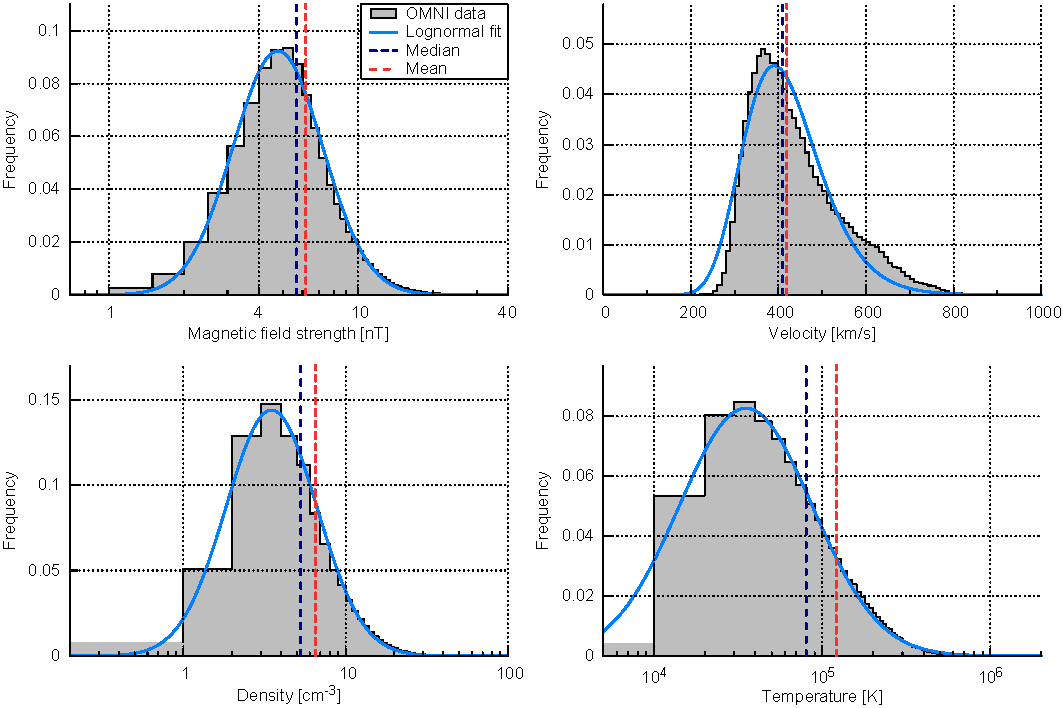
\includegraphics[width=1\textwidth]{images/gnuplots/histogram_fits_4_paper_pdfplot.pdf}
	\caption{The frequency distributions of the four solar wind parameters and their lognormal fits. The histograms have bins of 0.5~nT, 10~km/s, 1~cm$^{-3}$ and 10\,000~K and are based on the hourly OMNI data set. The fit's median and mean values are indicated as well.}
	\label{fig:histogram_fits_4_paper_pdfplot}
\end{figure}

%fit quality
From visual inspection, the resulting curves match well with the shape of the magnetic field strength, density and temperature distributions (\autoref{fig:histogram_fits_4_paper_pdfplot}). But for the velocity the fit function seems insufficient in describing its more complex shape.\\
From the normed stdfit values (\autoref{tab:single_lognormal_fit_parameters}) the velocity...\\

discuss high-value tail figures...\\

%gnuplot:
%sum of the squared differences or 'residuals' (SSR) between the input data points and the function values, evaluated at the same places. This quantity is often called 'chisquare' 
%'stdfit', the standard deviation of the fit, which is the rms of the residuals, and the variance of the residuals, also called 'reduced chisquare' when the data points are weighted.
%The 'sum of squares of residuals', also called 'chisquare', is the WSSR between the data and your fitted function; fit has minimized that.
%The WSSR can be used to calculate the reduced chisquare (WSSR/ndf) or stdfit, the standard deviation of the fit, sqrt(WSSR/ndf). Both of these are reported for the final WSSR.



%justification for compositional lognormal fit
To reach better fit results for the velocity the fit function has to be changed. We do not want to abandon the well-founded application of lognormal functions. But it is reasonable to assume that the distributions are composed of multiple branches (why?; slow/fast solar wind; literature; introduction). Therefore a compositional approach promises better fit results, which is why in the following we combine two lognormal functions.\\


\subsubsection{Double lognormal fit}

why only two? -> to keep it simple; every additional function adds further fit variables\\
compositional (two functions) lognormal regression fit\\

For the compositional regression fitting we use a function $W_\text{II}(x)$ which is composed of two lognormal distributions $W_1(x)$ and $W_2(x)$. The balancing parameter $c$ ensures that the resulting function remains normalized.
\begin{align}
	W_\text{II}(x) &= c \cdot W_1(x) + (1 -c) \cdot W_2(x)\\
	&= \frac{c}{\sigma_1 \sqrt{2 \pi} x} \, \text{e}^{- \frac{(\ln x - \mu_1)^2}{2 {\sigma_1}^2}} + \frac{(1 - c)}{\sigma_2 \sqrt{2 \pi} x} \, \text{e}^{- \frac{(\ln x - \mu_2)^2}{2 {\sigma_2}^2}} \label{eq:double_lognormal_fit_function}
\end{align}

The fitting of $W_\text{II}(x)$ to the frequency distributions gives the values of the five fit para\-meters ($c, \sigma_1, \mu_1, \sigma_2, \mu_2$), which are listed in \autoref{tab:double_lognormal_fit_parameters}.\\

The median of the composed distribution can be derived via solving
\begin{align}
	\int W_\text{II}(x)\,\text{d}x &= 0\\
	\intertext{and the mean via solving}
	\int x\,W_\text{II}(x)\,\text{d}x &= 0	\,.
\end{align}
Their values are listed in \autoref{tab:double_lognormal_fit_parameters}.
\begin{table}[htb]\small
	\centering
	\captionsetup{belowskip=4pt}
	\caption{These are the resulting fit coefficients from the double lognormal function (\ref{eq:double_lognormal_fit_function}) for the four examined solar wind parameters. The derived median and mean values are listed as well. Precision? Fit error in brackets.}
	\begin{tabular}{lcc.{2.8}.{1.8}ccccc}
		\toprule
		Parameter	&fkt	&\multicolumn{1}{c}{$c$}	&\multicolumn{1}{c}{$\mu$}	&\multicolumn{1}{c}{$\sigma$}	&\multicolumn{1}{c}{Median\up{a}}	&\multicolumn{1}{c}{Mean\up{a}}	&stdfit [$10^{-4}$]\\
		\midrule
		\multirow{2}{*}{Magnetic field}	&f1	&0.8656(79)	&1.7450(13)	&0.4631(23)	&\multirow{2}{*}{5.6570(X)}	&\multirow{2}{*}{6.769(X)}	&\multirow{2}{*}{3.1}\\
			&f2	&-	&1.6981(26)	&0.2061(50)	&	&	&\\
		\cmidrule{2-5}
		\multirow{2}{*}{Velocity}	&f1	&0.502(59)	&5.911(27)	&0.138(14)	&\multirow{2}{*}{413.4(X)}	&\multirow{2}{*}{439.1(X)}	&\multirow{2}{*}{6.6}\\
			&f2	&-	&6.1997(52)	&0.2117(40)	&	&	&\\
		\cmidrule{2-5}
		\multirow{2}{*}{Density}	&f1	&0.751(70)	&1.817(40)	&0.6970(88)	&\multirow{2}{*}{5.337(X)}	&\multirow{2}{*}{8.784(X)}	&\multirow{2}{*}{8.7}\\
			&f2	&-	&1.372(27)	&0.459(34)	&	&	&\\
		\cmidrule{2-5}
		\multirow{2}{*}{Temperature}	&f1	&0.669(11)	&10.9368(98)	&0.7691(54)	&\multirow{2}{*}{$8.081(X) \times 10^4$}	&\multirow{2}{*}{$1.667(X) \times 10^5$}	&\multirow{2}{*}{1.2}\\
			&f2	&-	&11.968(12)	&0.6007(42)	&	&	&\\
% 		Parameter	&\multicolumn{1}{c}{$c$}	&\multicolumn{1}{c}{$\mu_1$}	&\multicolumn{1}{c}{$\sigma_1$}	&\multicolumn{1}{c}{$\mu_2$}	&\multicolumn{1}{c}{$\sigma_2$}	&\multicolumn{1}{c}{Median\up{a}}	&\multicolumn{1}{c}{Mean\up{a}}	&stdfit [$10^{-4}$]\\
% 		\midrule
% 		Magnetic field	&0.8656(79)	&1.7450(13)	&0.4631(23)	&1.6981(26)	&0.2061(50)	&5.6570(X)	&6.769(X)	&3.1\\
% 		Velocity	&0.502(59)	&5.911(27)	&0.138(14)	&6.1997(52)	&0.2117(40)	&413.4(X)	&439.1(X)	&6.6\\
% 		Density		&0.751(70)	&1.817(40)	&0.6970(88)	&1.372(27)	&0.459(34)	&5.337(X)	&8.784(X)	&8.7\\
% 		Temperature	&0.669(11)	&10.9368(98)	&0.7691(54)	&11.968(12)	&0.6007(42)	&8.081(X) \times 10^4	&1.667(X) \times 10^5	&1.2\\
%data
% 		Magnetic field	&0.865639	&1.74495	&0.463091	&1.69810	&0.206097	&5.65690	&6.76908	&3.1\\
% 		Velocity	&0.501693	&5.91100	&0.138034	&6.19967	&0.211675	&413.374	&439.129	&6.6\\
% 		Density		&0.751122	&1.81740	&0.696961	&1.37232	&0.458973	&5.33677	&8.78361	&8.7\\
% 		Temperature	&0.669059	&10.9368	&0.769079	&11.9681	&0.600678	&80\,808.6	&166\,650	&1.2\\
%errors
% 		Magnetic field	&0.0079	&0.0013	&0.0023	&0.0026	&0.0050	&	&
% 		Velocity	&0.059	&0.027	&0.014	&0.0052	&0.0040	&	&
% 		Density		&0.070	&0.040	&0.0088	&0.027	&0.034	&	&
% 		Temperature	&0.011	&0.0098	&0.0054	&0.012	&0.0042	&	&
		\bottomrule
		\multicolumn{5}{l}{\footnotesize{\up{a}Values in their respective units nT, km/s, cm$^{-3}$ and K.}}
	\end{tabular}
	\label{tab:double_lognormal_fit_parameters}
\end{table}

The fitted functions show [a good match] for the parameters, [even for the velocity] (see Figure~XX).\\
how good fits the function to the shape? discuss figures...
\begin{figure}[htb]
	%\centering
	\fcapside[\FBwidth]{
		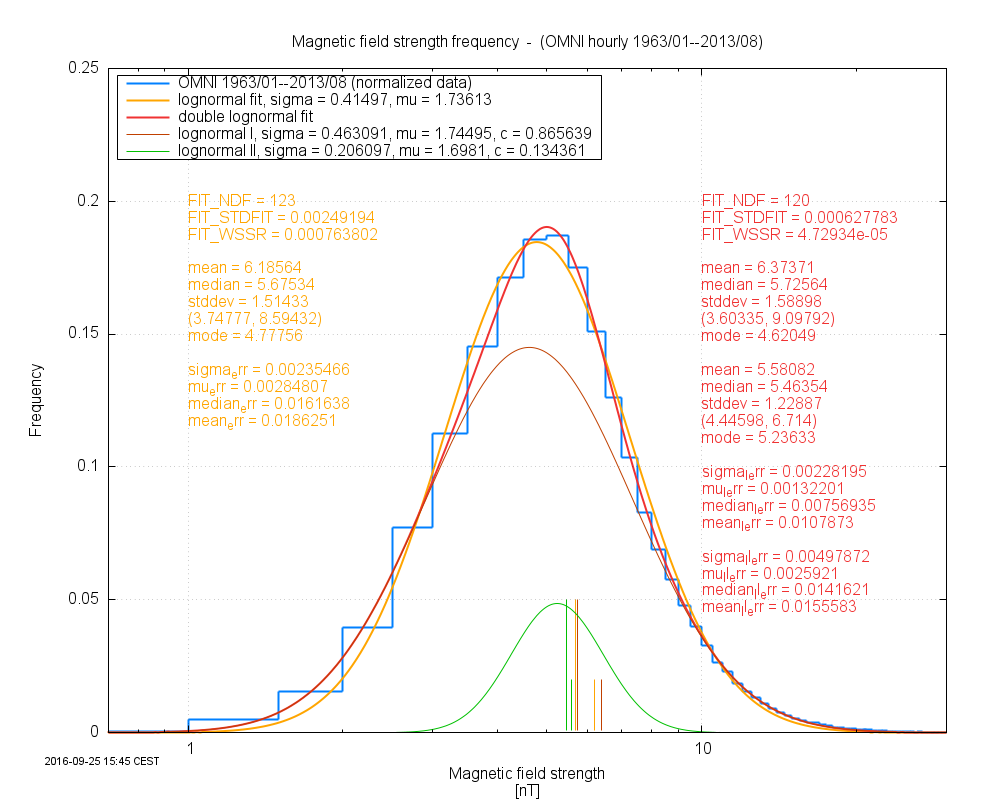
\includegraphics[width=0.3\textwidth]{images/gnuplots/histogram_B_frequency_fit_plot.png}
	}{
		\caption{Plot of the double lognormal fit on the magnetic field strength frequency distribution. 3:2}
		\label{fig:histogram_B_frequency_fit_plot_DOUBLE}
	}
\end{figure}

goodness of fit; discuss high value zoom figures\\


%goodness of fit comparison
To be able to compare the goodness of the single with the compositional lognormal fits we make use of their corresponding sum of squared residuals (SSR). More precisely the 'reduced SSR' where the SSR is divided by the number of degrees of freedom to account for the data set size and the fit function complexity (for more on SSRs see Appendix \autoref{sec:goodness_of_fit}). As anticipated, the reduced SSR values of the composed fit are considerably smaller. The evaluation of the ratio of the reduced SSRs of the respective single and double fits shows that indeed the double fits are 3.7--19.1 times more accurate (see \autoref{tab:shape_ssr_comparison}).
\begin{table}[htb]\small
	\centering
	\ttabbox{
	\captionsetup{belowskip=4pt}
	\caption{The reduced SSR for the single and the double lognormal fit and their ratio. use stdfit for comparison...}
	\label{tab:shape_ssr_comparison}
	}{
	\begin{tabular}{l S[table-figures-exponent=4] S[table-figures-exponent=4] S}
		\toprule
		Parameter	&\multicolumn{1}{c}{single SSR$_\text{red}$}	&\multicolumn{1}{c}{double SSR$_\text{red}$}	&\multicolumn{1}{c}{ratio s/d}\\
		\midrule
		Magnetic field	&7.64e-4	&4.73e-5	&16.15\\
		Velocity	&8.41e-6	&4.41e-7	&19.07\\
		Density		&3.23e-4	&8.67e-5	&3.73\\
		Temperature	&8.34e-13	&8.97e-14	&9.30\\
% 		Magnetic field strength	&7.64 \times 10^{-4}	&4.73 \times 10^{-5}	&16.15\\
% 		Velocity		&8.41 \times 10^{-6}	&4.41 \times 10^{-7}	&19.07\\
% 		Density			&3.23 \times 10^{-4}	&8.67 \times 10^{-5}	&3.73\\
% 		Temperature		&8.34 \times 10^{-13}	&8.97 \times 10^{-14}	&9.30\\
		\bottomrule
	\end{tabular}
	}
\end{table}


%discussion of comparison-table 
Especially the velocity and the magnetic field strength benefit from the more complex fit function.\\
When is the single fit sufficient? -> maybe evaluate from absolute goodness of fit...\\


\subsection{Helios solar wind model}

Helios data, radial binned and frequency binned\\
Fit on the solar distance and frequency using the balancing parameter $c$ from the compositional shape fit before (see equation~(\ref{eq:double_lognormal_fit_function})).\\
=> fit function with solar distance dependency\\
to be able to make the model's radial dependency exponential, we fit not $\mu$ and $\sigma$ but the median ($\tilde{x}, x^\text{med}, x_\text{med}, \xi$?) and mean ($\bar{x}$) of both lognormal functions to the data. As these parameters can be derived from each other directly, equation (\ref{eq:double_lognormal_fit_function}) with the replacing relations\\
\begin{align}
	\tilde{x} &= \text{e}^{\mu}	&	&\Longrightarrow	&	\mu &= \ln(\tilde{x})\\
	\bar{x} &= \text{e}^{(\mu + \frac{\sigma^2}{2})}	&	&\Longrightarrow	&	\sigma &= \sqrt{2 \ln\left(\frac{\bar{x}}{\tilde{x}}\right)}
\end{align}
results in
\begin{align}
	W_\text{II}(x,\tilde{x}_1,\bar{x}_1,\tilde{x}_2,\bar{x}_2) = \frac{c}{2 \sqrt{\pi \ln\left(\frac{\bar{x}_1}{\tilde{x}_1}\right)} \, x} \, \exp\left(- \frac{\ln^2\left(\frac{x}{\tilde{x}_1}\right)}{4 \ln\left(\frac{\bar{x}_1}{\tilde{x}_1}\right)}\right) + \frac{(1 - c)}{2 \sqrt{\pi \ln\left(\frac{\bar{x}_2}{\tilde{x}_2}\right)} \, x} \, \exp\left(- \frac{\ln^2\left(\frac{x}{\tilde{x}_2}\right)}{4 \ln\left(\frac{\bar{x}_2}{\tilde{x}_2}\right)}\right)
\end{align}
introducing the radial exponential dependency of the mean and median\\
\begin{align}
	\tilde{x}_1(r) = \tilde{a}_1 \, r^{\tilde{b}_1}\\
	\bar{x}_1(r) = \bar{a}_1 \, r^{\bar{b}_1}\\
	\tilde{x}_2(r) = \tilde{a}_2 \, r^{\tilde{b}_2}\\
	\bar{x}_2(r) = \bar{a}_2 \, r^{\bar{b}_2}
\end{align}
we get the ultimate monster equation:\\
\begin{align}
	W_\text{II}(x,\tilde{a}_1, \tilde{b}_1, \bar{a}_1, \bar{b}_1, \tilde{a}_2, \tilde{b}_2, \bar{a}_2, \bar{b}_2) =\\
	\frac{c}{2 \sqrt{\pi \ln\left(\frac{\bar{a}_1 \, r^{\bar{b}_1}}{\tilde{a}_1 \, r^{\tilde{b}_1}}\right)} \, x} \, \exp\left(- \frac{\ln^2\left(\frac{x}{\tilde{a}_1 \, r^{\tilde{b}_1}}\right)}{4 \ln\left(\frac{\bar{a}_1 \, r^{\bar{b}_1}}{\tilde{a}_1 \, r^{\tilde{b}_1}}\right)}\right) + \frac{(1 - c)}{2 \sqrt{\pi \ln\left(\frac{\bar{a}_2 \, r^{\bar{b}_2}}{\tilde{a}_2 \, r^{\tilde{b}_2}}\right)} \, x} \, \exp\left(- \frac{\ln^2\left(\frac{x}{\tilde{a}_2 \, r^{\tilde{b}_2}}\right)}{4 \ln\left(\frac{\bar{a}_2 \, r^{\bar{b}_2}}{\tilde{a}_2 \, r^{\tilde{b}_2}}\right)}\right)
\end{align}



the model represents the data well, see \autoref{fig:double_fit_B_freq_r_004au_plot_thesis}\\
\begin{figure}[htb]
	\centering
	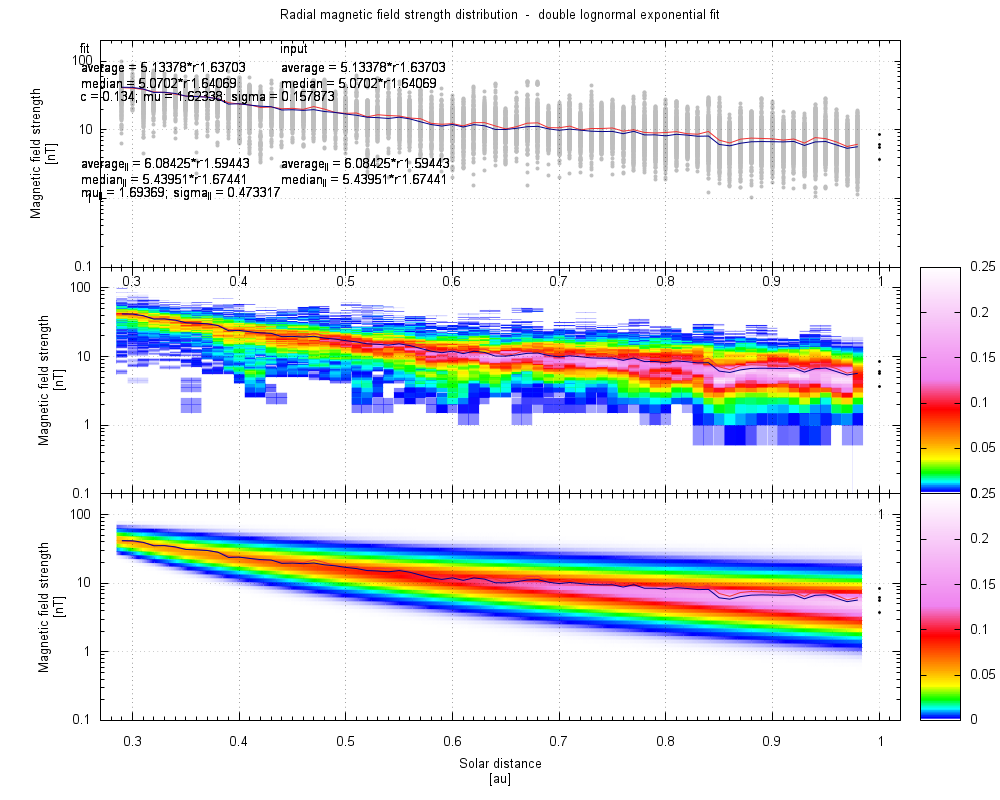
\includegraphics[width=0.4\textwidth]{images/gnuplots/double_fit_B_freq_r_004au_plot_thesis.png}
	\caption{Plot of the magnetic field strength over solar distance. The top panel shows the hourly data from both Helios spacecraft, their median and their mean values. The second panel shows the same data binned into 0.1~au and 0.5~nT bins. The bins are normalized for distance, i.e. the bin values represent the frequency of getting the bin magnitude at that distance. The bottom panel shows the exponential double lognormal function (XX), which is obtained from fitting to the data. insert keys... adjust color scale... keep log x scale?}
	\label{fig:double_fit_B_freq_r_004au_plot_thesis}
\end{figure}

The resulting fit coefficients for all four solar wind parameters are presented in \autoref{tab:helios_model_fit_parameters}.
\begin{table}[htb]\small
	\centering
	\captionsetup{belowskip=4pt}
	\caption{These are the resulting fit coefficients from the compositional function (XX). precision... Fit error in brackets? 2-line table if fit errors do not reduce it enough...}
	\begin{tabular}{lcccccccccccc}
		\toprule
		\multirow{3}{*}{Plasma parameter}	&	&\multicolumn{5}{c}{$W_1(x,r)$}	&	&\multicolumn{5}{c}{$W_2(x,r)$}\\
		\cmidrule{3-7}	\cmidrule{9-13}
			&$c$	&\multicolumn{2}{c}{median}	&	&\multicolumn{2}{c}{mean}	&	&\multicolumn{2}{c}{median}	&	&\multicolumn{2}{c}{mean}\\
		\cmidrule{3-4}	\cmidrule{6-7}	\cmidrule{9-10}	\cmidrule{12-13}
			&	&$a$	&$b$	&	&$a$	&$b$	&	&$a$	&$b$	&	&$a$	&$b$\\
		\midrule
		Magnetic field strength	&0.866	&5.43951	&-1.67441	&	&6.08425	&-1.59443	&	&5.0702	&-1.64069	&	&5.13378	&-1.63703\\
		Velocity		&0.502	&370.994	&0.114544	&	&373.556	&0.107352	&	&480.016	&-0.0151313	&	&494.135	&-0.0207186\\
		Density		&0.751	&6.75345	&-2.17915	&	&8.13399	&-2.19658	&	&3.09089	&-2.12598	&	&3.42042	&-2.08600\\
		Temperature		&0.669	&41\,262.8	&-1.18491	&	&58\,852.7	&-1.32940	&	&141\,238	&-0.570392	&	&168\,399	&-0.520731\\
% 		Plasma parameter	&$c$	&$\mu_1$	&$\sigma_1$	&$\mu_2$	&$\sigma_2$\\
% 		\midrule
% 		Magnetic field strength	&0.866	&1.69369	&0.473315	&1.62338	&0.157874\\
% 		Velocity		&0.502	&5.91619	&0.117315	&6.17382	&0.240790\\
% 		Density		&0.751	&1.91005	&0.609916	&1.12846	&0.450123\\
% 		Temperature		&0.669	&10.6277	&0.842705	&11.8582	&0.593111\\
		\bottomrule
	\end{tabular}
	\label{tab:helios_model_fit_parameters}
\end{table}

The model's amplitude differences to the data are becoming larger with smaller solar distance (check it.), see \autoref{fig:double_fit_B_freq_r_plot_thesis}\\
\begin{figure}[htb]
	\centering
	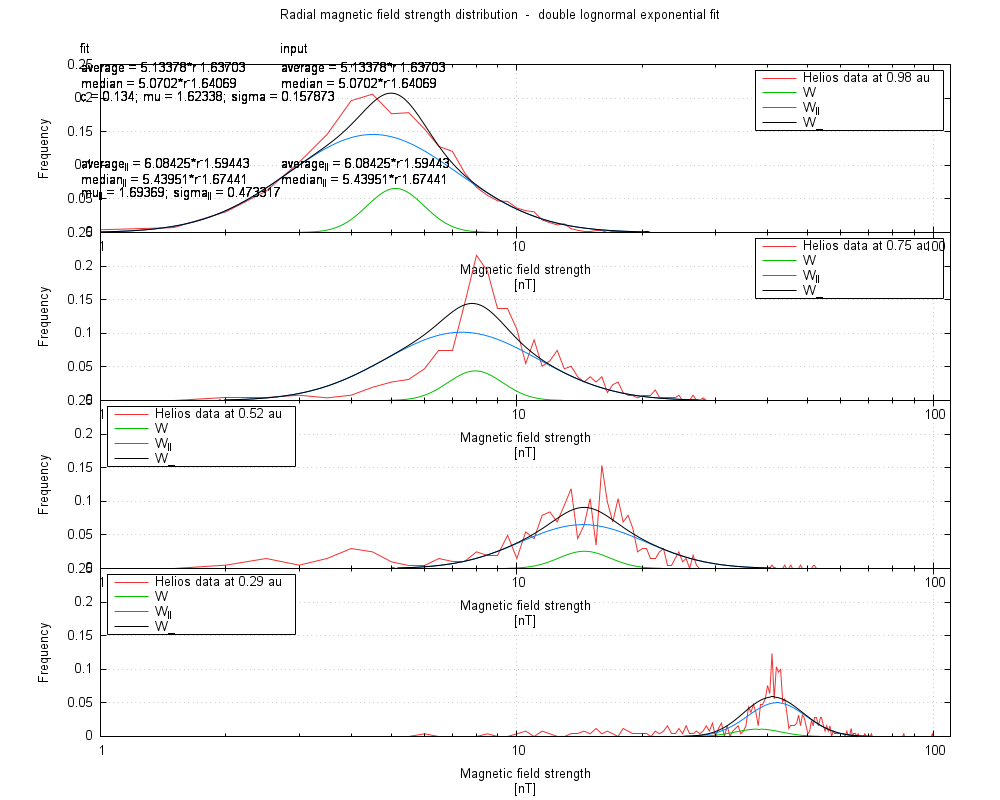
\includegraphics[width=0.4\textwidth]{images/gnuplots/double_fit_B_freq_r_plot_thesis.png}
	\caption{Plot of the magnetic field strength's frequency distribution at different solar distances (0.29, 0.52, 0.75 and 0.98~au). The Helios data, the composed fit model and both its components are plotted. 0.23~au steps, lw 2, stepfunction}
	\label{fig:double_fit_B_freq_r_plot_thesis}
\end{figure}


comparison with simple radial mean and median\\

%%%%%%%%%%%
The distribution width varies with heliospheric distance (back up with figure!).\\

We see that the density and temperature shapes stay almost constant...\\

varying shape with distance is indicator for internal physical processes (mixing/turbulence...)\\


\subsubsection{Model quality}

self-consistency?; model assumptions valid?\\

limitations: The model is valid within the heliospheric distance range of 0.29--0.98~au in the ecliptic plane (with maximal errors of...). average hourly values.\\

validity and estimation of error size outside of valid model range...\\
spatial ranges:\\
- radial range of model validity (extrapolation boundaries)\\
- latitude range...\\

Model extrapolation to near-Sun region (and Mars orbit?)\\

expanding the range of the model to the Sun leads to a singularity, see \autoref{fig:double_fit_B_freq_r_004au_plot}
\begin{figure}[htb]
	\centering
	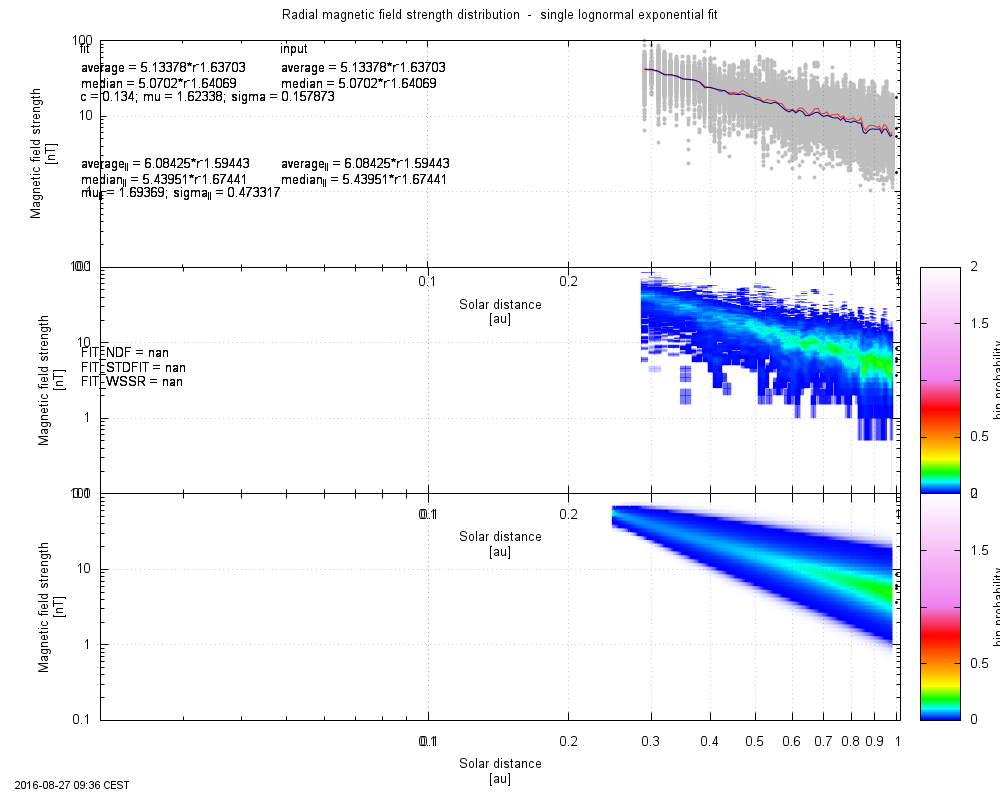
\includegraphics[width=0.4\textwidth]{images/gnuplots/double_fit_B_freq_r_004au_plot.png}
	\caption{expanding the range of the model to the Sun leads to a singularity... expand range to >2~au...}
	\label{fig:double_fit_B_freq_r_004au_plot}
\end{figure}
that is caused by the convergence and eventually crossing of median(r) and mean(r)\\

%argument for constant width function
for the magnetic field strength the mean and median cross each other at 0.246~au. below that point it cannot be lognormally distributed anymore, because for lognormal functions always applies mean > median (see Section~XX)\\
=> what kind of distribution has the B-field near the Sun?\\

%crossing distances:
% B: W1: 0.246466~au\\
% W2: 0.0332098\\
% v: W1: 2.603616\\
% W2: 179.1872517\\
% n: W1: 43094.3434\\
% W2: 0.0793510\\
% T W1: 11.674953\\
% W2: 0.0289609\\

\section{Extrapolation model}

for the extrapolation it is better to use a single lognormal function, because:\\
- extrapolation error so big that additional accuracy would not matter\\
- [easier to compute the mean(r) and median(r); otherwise numerical determination]\\
- model easier to modify for different time ranges\\
- ...\\
new requirement: possibility to extrapolate the model to the near-Sun region\\
to avoid the crossing of median(r) and mean(r), their exponents $b$ have to be identical (constant width)\\
$median(r) = X_{\text{med},0} r^b$\\
$mean(r) = mean_0 r^b$\\
fit function here...\\
So the new fit function has only the three fit parameters $median_0, mean_0$ and $b$.\\

The resulting fit coefficients for all solar wind parameters are presented in \autoref{tab:extrapolation_model_fit_parameters}.
\begin{table}[htb]\small
	\centering
	\captionsetup{belowskip=4pt}
	\caption{The resulting fit coefficients from the single lognormal fit of function (XX). constant width... Standard fit error in brackets.}
	\begin{tabular}{l.{3.13}.{3.13}.{2.8}}
		\toprule
		Parameter	&\multicolumn{1}{c}{$\tilde{x}_0$\up{a}}	&\multicolumn{1}{c}{$\bar{x}_0$\up{a}}	&\multicolumn{1}{c}{$b$}\\
		\midrule
		Magnetic field	&5.358(25)	&5.705(28)	&-1.662(11)\\
		Velocity	&399.1(17)	&411.7(18)	&0.0711(71)\\
		Density		&5.424(33)	&6.845(47)	&-2.114(20)\\
		Temperature	&6.357(64) \times 10^4	&1.072(14) \times 10^5	&-1.100(20)\\
% 		Magnetic field	&5.35847~nT	&5.70494~nT	&-1.66152\\
% 		Velocity		&399.080~km/s	&411.699~km/s	&0.0710568\\
% 		Density			&5.42431~cm$^{-3}$	&6.84454~cm$^{-3}$	&-2.11388\\
% 		Temperature		&63\,570.7~K	&107\,224~K	&-1.10001\\
% 		Magnetic field	&0.025	&0.028	&0.011\\
% 		Velocity	&1.7	&1.8	&0.0071\\
% 		Density		&0.033	&0.047	&0.015\\
% 		Temperature	&640	&1390	&0.020\\
		\bottomrule
		\multicolumn{4}{l}{\footnotesize{\up{a}Values in their respective units nT, km/s, cm$^{-3}$ and K.}}
	\end{tabular}
	\label{tab:extrapolation_model_fit_parameters}
\end{table}

frequency distribution, see \autoref{fig:single_fit_B_freq_r_plot_const_width}
\begin{figure}[htb]
	\centering
	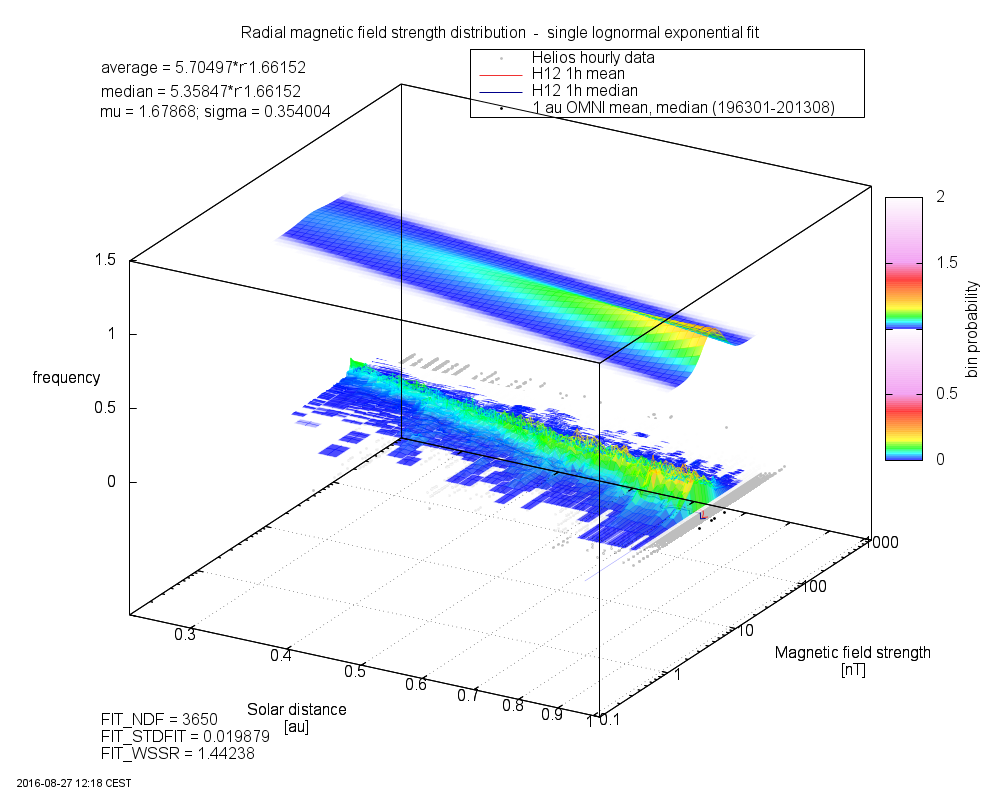
\includegraphics[width=0.4\textwidth]{images/gnuplots/single_fit_B_freq_r_plot_const_width.png}
	\caption{remove 3d plot, make 2d Plot of the magnetic field strength's frequency distribution at different solar distances (0.29, 0.52, 0.75 and 0.98~au). The Helios data and the single lognormal fit model with constant width are plotted. 0.23~au steps, stepfunction}
	\label{fig:single_fit_B_freq_r_plot_const_width}
\end{figure}

single fit model with constant width, see \autoref{fig:single_fit_fixed_4_thesis_plot}
\begin{figure}[htb]
	\centering
	\includegraphics[width=0.4\textwidth]{images/gnuplots/single_fit_fixed_4_thesis_plot.pdf}
	\caption{The solar wind parameter's frequency distribution over solar distance. The Helios data and the single lognormal fit model with constant width are plotted.}
	\label{fig:single_fit_fixed_4_thesis_plot}
\end{figure}

%error discussion
W error\\
B stdfit error: 0.020\\
B error at (1~au,Bmean): 0.011\\
B error at (1~au,Bmedian): 0.011\\
max data $-$ model deviation: 0.011\\

see \autoref{fig:single_fit_B_freq_r_004au_plot_const_width}
\begin{figure}[htb]
	\centering
	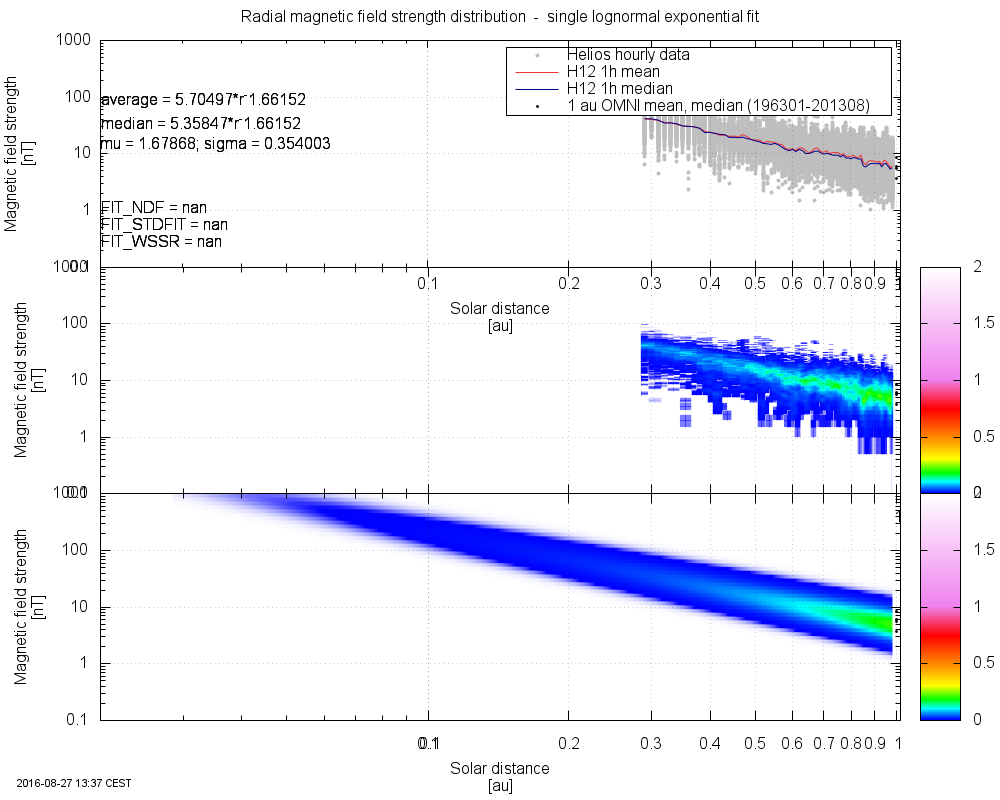
\includegraphics[width=0.4\textwidth]{images/gnuplots/single_fit_B_freq_r_004au_plot_const_width.png}
	\caption{Plot of the magnetic field strength over solar distance (similar to Figure~XX). The top panel shows the same data binned into 0.1~au and 0.5~nT bins. The bins are normalized for distance, i.e. the bin values represent the frequency of getting the bin magnitude at that distance. The bottom panel shows the exponential single lognormal function (XX) with constant width, which is obtained from fitting to the data. insert keys... adjust color scale... keep log x scale? remove top panel...}
	\label{fig:single_fit_B_freq_r_004au_plot_const_width}
\end{figure}

quartile fit extrapolation...\\

expected values at 0.04~au...\\


\subsection{Model validity}

validity and estimation of error size outside of valid model range...\\

The extrapolation distance is only about one third of the model range, but as the parameters follow exponential change, one has to look at the logarithmic distance which is indeed one and a half times the model range.\\

argument with gravitational deceleration; near-Sun extrapolation should be biased, because in the near-Sun region gravitation becomes significant (see \autoref{fig:v_vs_r_b})\\
\begin{figure}[htb]
	\centering
	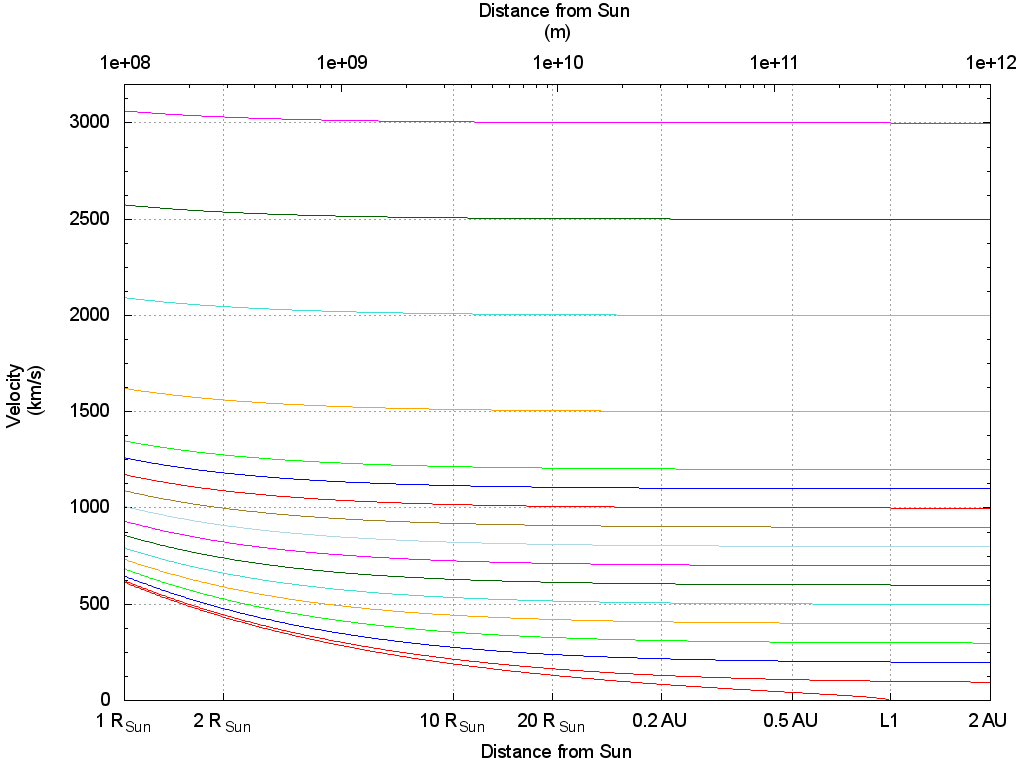
\includegraphics[width=0.3\textwidth]{images/gnuplots/v_vs_r_b.png}
	\caption{velocity over solar distance; gravitational deceleration. place instead figure of grav. force over solar distance...}
	\label{fig:v_vs_r_b}
\end{figure}

polar plot with highlighted model range and 1-3 extrapolation extensions... (for both models)\\


\subsection{Model comparison via SSR}

model comparison via the reduced SSR for the fit parameters from Tables~\ref{tab:extrapolation_model_fit_parameters} and \ref{tab:helios_model_fit_parameters}, see \autoref{tab:model_ssr_comparison}\\
\begin{table}[htb]\small
	\centering
	\captionsetup{belowskip=4pt}
	\caption{The reduced SSR for the Helios model and the extrapolation model fits and their ratio. precision...}
	\begin{tabular}{l>{$}l<{$}>{$}l<{$}c}
		\toprule
		Plasma parameter	&$Helios model $SSR_\text{red}	&$Extrapolation model $SSR_\text{red}	&ratio Helios/extrapolation\\
		\midrule
		Magnetic field strength	&1.18			&1.44			&1.22\\
		Velocity		&2.66 \times 10^{-3}	&3.47 \times 10^{-3}	&1.30\\
		Density			&2.54 \times 10^{-1}	&2.67 \times 10^{-1}	&1.05\\
		Temperature		&2.14 \times 10^{-9}	&2.35 \times 10^{-9}	&1.10\\
% 		Magnetic field strength	&1.17979		&1.44238		&1.223\\
% 		Velocity		&2.66309 \times 10^{-3}	&3.47353 \times 10^{-3}	&1.304\\
% 		Density			&0.254132		&0.26671		&1.049\\
% 		Temperature		&2.13713 \times 10^{-9}	&2.34673 \times 10^{-9}	&1.098\\
		\bottomrule
	\end{tabular}
	\label{tab:model_ssr_comparison}
\end{table}


\subsection{Adjusted extrapolation models}

extrapolation models for different time spans:\\
extrapolation with OMNI data and solar cycle/seasonal variations\\


\subsection{Comparison with existing extrapolation models}

comparison with s.o. elses values...\\
...with Vourlidas estimates at 10~$R_\odot$\\
...with Wang2000 slow blobs\\


\section{Radial evolution of solar wind structures}

%see CGAUSS report2015_2

Radial evolution of solar wind structures from Helios data\\

Helios event lists HSSs, SLOWs, CIRs, CMEs...; event lists for all Helios data\\
see Liu2004 for Helios ICME list and radial dependencies of B, n, T and v...\\

200~km/s slow solar wind at 10~$R_\odot$ is in agreement with blob measurements from Wang2000\\

very slow sw (VSSW) gets accelerated; see Sanchez-Diaz2016:\\
%"The reported in situ measurements suggest that the properties of VSSW are a continuation of the slow wind toward lower speeds: higher densities, higher proton fluxes, and lower temperatures, thereby extending well-known scaling laws [Lopez and Freeman, 1986; Hundhausen et al., 1970] down to speeds as low as 200 km/s."\\
%"The VSSW has a number of interesting properties that suggest it may be the interplanetary signature of long HPS crossings."\\

structure extrapolations\\

radial diameter of MCs increase between 0.3~au and 4.3~au proportional to the distance as $r^{0.8}$ \citep{Bothmer1998}\\

MC central axial magnetic field strength radial density dependence $B = 18.1\,r^{-1.64}$ \citet{Leitner2007}\\
MC average diameter $D = 0.23\,r^{1.14}$ \citet{Leitner2007}

sw structure marked plot\\


\section{Summary/Results}

where does the solar wind get accelerated? (at 3--4~Rs for moving density enhancements (slow solar wind), see Sheeley1997)\\
results beneficial for Solar~Probe~Plus (SPP) mission which is to investigate coronal heating and the origin of the solar wind\\
SPP will have its closest perihelion at 9.86~solar radii (0.0459~au), see \citet{Fox2015}\\
